\documentclass[10pt, conference]{IEEEtran}
\IEEEoverridecommandlockouts
% The preceding line is only needed to identify funding in the first footnote. If that is unneeded, please comment it out.
\usepackage{cite}
\usepackage{amsmath,amssymb,amsfonts}
\usepackage{algorithm}
% \usepackage{algorithmic}
\usepackage{algpseudocode}
\usepackage{graphicx}
\usepackage{textcomp}
\usepackage{xcolor}
\usepackage{bm}
\usepackage{subcaption}
\usepackage{float}
\usepackage{afterpage}
\usepackage[acronym]{glossaries}
\def\BibTeX{{\rm B\kern-.05em{\sc i\kern-.025em b}\kern-.08em
    T\kern-.1667em\lower.7ex\hbox{E}\kern-.125emX}}


\makeglossaries

\newacronym{fp}{FP}{false positive}
\newacronym{fn}{FN}{false negative}
\newacronym{fna}{FNA}{fine needle aspirate}
\newacronym{oob}{OOB}{out-of-bag}
\newacronym{sse}{SSE}{sum of squared error}
\newacronym{tp}{TP}{true positive}

\begin{document}

\title{Assignment 3 Option 2 \\
Quantity To Produce Quality
}

\author{\IEEEauthorblockN{A.D. van der Merwe}
\IEEEauthorblockA{Department of Computer Science \\
University of Stellenbosch\\
24923273 \\
24923273@sun.ac.za}
}

\maketitle

\begin{abstract}
This paper investigates the influence of the size of the bags, the number of randomly selected features and
the number of members in linear and non-linear logistic regression ensemble models. Both the ensemble models
are applied to classify five binary classification datasets that vary in complexity. The non-linear logistic
regression ensemble can capture non-linear relationships between descriptive features in a dataset, which
generally allows it to perform better than the linear logistic regression ensemble model. The size of the bags,
the number of randomly selected features, and the number of ensemble members are highly problem-dependent and
should all be considered together to optimise model performance on a given dataset.
\end{abstract}

\section{Introduction}

Three critical parameters that must be optimised in an ensemble model are the size of the bags,
the number of randomly selected features and the number of members in linear and non-linear logistic
regression ensembles. Each of these parameters can significantly influence the performance of the ensemble
if inappropriate values are selected.

This paper investigates the influence of the size of the bags, the number of randomly selected features and
the number of members in linear and non-linear logistic regression ensemble models across five binary classification
datasets that varies in complexity.

The non-linear logistic regression ensemble model generally performed better than the linear logistic regression
ensemble model, as the non-linear ensemble was able to capture more complex relationships between descriptive
features in the datasets. To create an optimal ensemble of a dataset, the size of the bags, the number of
randomly selected features, and the number of members should all be considered together. All of these elements
significantly influence how well the ensemble performs.

The rest of this paper is structured as follows: Section \ref{section: Background} provides background
information on gradient descent optimisation, the logistic regression model, basis functions, ensemble learning.
Additionally, background on bootstrap aggregating and the performance metrics used in this paper.
Section \ref{section: Implementation} provides the implementation of the linear and non-linear logistic
regression ensemble models. Section \ref{section: Empeirical Procedure} provides the empirical procedure and Section
\ref{section: Research Results} provides the research results.

\section{Background} \label{section: Background}

This section presents background information on the gradient descent optimisation algorithm, logistic
regression model, and ensemble learning. Additionally, background information on bootstrap aggregating,
basis functions, and performance metrics used in this report.

\subsection{Gradient Descent}

The gradient descent algorithm was first introduced by Augustin-Louis Cauchy
in 1847 \cite{gradient_descent_ref}. Cauchy introduced gradient descent to solve optimisation
systems of simultaneous equations through iterative optimisation to find the minimum of a function.
Cauchy also introduced the step size parameter, now commonly referred to as the learning rate, to control
how large the steps are for each iteration as the algorithm updates model parameters to reach an optimal
solution.

The generic learning algorithm of gradient descent is represented by Algorithm \ref{alg:GDLA_algorithm}.
\begin{algorithm}[H]
    \caption{Gradient Descent Learning Algorithm}
    \label{alg:GDLA_algorithm}
    \begin{algorithmic}[1]
        \State Preprocess the training set $D_T$ as necessary
        \State Initialise parameter vector, \textbf{w}$(t)$, $t=0$
        \State Initialise the learning rate $\eta$
        \While{stopping condition not satisfied}
            \For{each $i = 1,...,n_T$}
                \State Calculate error signal, $\delta(t)$
                \State Calculate a search direction, \textbf{q}$(t) = f\left( \text{\textbf{w}}(t), \delta(t) \right)$
                \State Update parameter vector: \textbf{w}$(t+1) = \text{\textbf{w}}(t) + \eta \text{\textbf{q}}(t)$
            \EndFor
            \State $t = t + 1$
            \State Compute prediction error
        \EndWhile
        \State Return \textbf{w}$(t-1)$ as solution
    \end{algorithmic}
\end{algorithm}

\subsection{Logistic Regression} \label{section: logistic_regression_background}

The logistic regression model was first introduced by David Cox in 1958 as a method to perform binary
classification \cite{logistic_regression_ref}. Cox specifically designed the logistic regression
model to model the probability of a binary outcome as a function of descriptive features.

To construct a logistic regression model that makes use of gradient descent as an optimisation
algorithm, a threshold function that is continuous, and therefore differentiable is needed. This function
is known as the logistic function and is represented by the mathematical equation below.
\begin{equation}
    Logistic(z) = \frac{1}{1 + e^{-z}} \label{eq: logistic_function}
\end{equation}
where $z$ is a numeric value.

Before the logistic regression model is constructed the binary target features are mapped to 0 or 1.
The logistic regression model is then constructed by use of the equation that follows.
\begin{equation}
    \mathbb{M}_{\textbf{w}}(\textbf{d}_i) = \frac{1}{1 + e^{-\textbf{w} \cdot \textbf{d}_i}} \label{eq: logistic_regression_equation}
\end{equation}
where $\textbf{d}_i$ is a vector of the $i$-th descriptive features, with the bias term represented by $\textbf{d}_0$ and equal to one,
\textbf{w} is a vector of weights, where $\textbf{w}_0$ represents the weight of the bias term, and the weights that remain corresponds
to their respective descriptive features in $\textbf{d}_i$. The term $\mathbb{M}_{\textbf{w}}(\textbf{d}_i)$ represents the predicted output
for the $i$-th instance of the logistic regression model. The output of the logistic regression model can be interpreted as probabilities
of the occurrence of a target instance that belongs to a specific class. The probability the $i$-th target instance that belongs to class one
is given by the equation below.
\begin{equation}
    P(y_i = 1|\textbf{d}_i) = \mathbb{M}_{\textbf{w}}(\textbf{d}_i) \label{eq: classified_class_1}
\end{equation}
where $y_i$ is the true label for the $i$-th observation. Similarly, the probability of the $i$-th target instance that belongs to class
zero is given by the equation below.
\begin{equation}
    P(y_i = 0|\textbf{d}_i) = 1 - \mathbb{M}_{\textbf{w}}(\textbf{d}_i) \label{eq: classified_class_0}
\end{equation}

To classify the $i$-th target instance, $\mathbb{M}_{\textbf{w}}(\textbf{d}_i)$ is compared to a threshold of $0.5$. The equation used
to classify the $i$-th target feature that belongs to either class zero or class one is given as follows.
\begin{equation}
    \hat{y}_i = 
    \begin{cases}
    0 & \text{if } \mathbb{M}_{\textbf{w}}(\textbf{d}_i) < 0.5 \\
    1 & \text{if } \mathbb{M}_{\textbf{w}}(\textbf{d}_i) \geq 0.5 
    \end{cases}
    \label{eq: classify_target_instance}
\end{equation}
where $\hat{y}_i$ is the predicted class of the $i$-th binary target variable.

Gradient descent is used as the optimisation algorithm to find the optimal decision boundary for a logistic regression model.
The optimal decision boundary is defined as the set of weights that minimise the \acrfull{sse} based on the training set.
The mathematical represntation of the \acrshort{sse} is as follows.
\begin{equation}
    L_2\left(\mathbb{M}_{\textbf{w}}, \mathcal{D}\right) = \frac{1}{2} \sum_{i=1}^{n} \left( y_i - \mathbb{M}_{\textbf{w}}(\textbf{d}_i) \right)^2 \label{eq: sse_function}
\end{equation}
where $\mathcal{D}$ is the training dataset and $n$ is the number of instances in the training dataset and $L_2$ is the
\acrshort{sse} of the training dataset.

The equation used to represent the error signal used in the gradient descent optimisation algorithm to update the weights
of the logistic regression model is as follows.
\begin{equation}
    \delta(\mathcal{D}, w_j) = \sum_{i=1}^{n} \left((y_i - \mathbb{M}_{\textbf{w}}(\textbf{d}_i)) \mathbb{M}_{\textbf{w}}(\textbf{d}_i)
                                    (1-\mathbb{M}_{\textbf{w}}(\textbf{d}_i)) d_{i,j}\right) \label{eq: error_signal}
\end{equation}
where $w_j$ is the $j$-th weight of the logistic regression model and $d_{i,j}$ is the value of the $j$-th
feature for the $i$-th instance of the training dataset.

The equation used to update the weights of the logistic regression model by use of the gradient descent optimisation algorithm
is as follows.
\begin{equation}
    w_j = w_j + \eta \sum_{i=1}^{n} \left((y_i - \mathbb{M}_{\textbf{w}}(\textbf{d}_i)) \mathbb{M}_{\textbf{w}}(\textbf{d}_i)
                            (1-\mathbb{M}_{\textbf{w}}(\textbf{d}_i)) d_{i,j}\right) \label{eq: weight_update}
\end{equation}
where $\eta$ is the learning rate.

The logistic regression model is quite robust to noise and outliers in the dataset. However, the logistic
regression can not handle missing values and sensitive to imbalanced classes. Additionally, the logistic
regression model requires categorical features to be encoded into numerical representation by either the
ordinal encoded or the one hot encoded technique and the data needs to be scaled or normalised. Feature subset
selection also applies, as logistic regression tends to overfit on data with a large number of features.
The logistic regression also assumes a linear relationship between the descriptive
features, where the actual relationship between descriptive features might be non-linear.

\subsection{Basis Functions} \label{section: basis_functions_background}

Basis functions are non-linear elements which transforms the linear inputs to the logistic regression
into non-linear represntations, while the model itself remains linear in terms of the weights \cite{basis_fun_ref}.
The addition of basis functions allows logistic regression model to capture relationships between descriptive
features which are non-linear.

The data is transformed by use of a series of basis functions, which enables the logistic regression model to effectively
manage non-linear relationships between descriptive features. A logistic regression model that makes use of
basis functions is represented by the equation below.
\begin{equation}
    \mathbb{M}_{\textbf{w}}(\textbf{d}_i) = \frac{1}{1 + e^{-\sum_{j=0}^{b}w_j \phi_j(\textbf{d}_i)}} \label{eq: non_logistic_regression_equation}
\end{equation}
where $\phi_0$ to $\phi_b$ are a series of $b$ basis functions that each transform the $i$-th input vector $\textbf{d}_i$ in a different way.
Usually $b$ is larger than $n$, which means that there are more basis functions than there are descriptive features.

There are two main disadvantages when basis functions are used in a logistic regression model to capture non-linear relationships
between descriptive features. Firstly, some prior knowledge of these non-linear relationships is required to select appropriate
basis functions. Secondly, an increased number of basis functions results in larger gradient descent search spaces, which can lead to
longer convergence times and complicate the optimisation process.

\subsection{Ensemble Learning}

Ensemble learning combines several individual models to to obtain better generalisation performance and predict a new instance
based on multiple models opposed to a single model \cite{Ensemble_ref}.

Each model in an ensemble is trained on the same dataset and yields slightly different results due to variations
in training data, model configurations or model architectures. Each model performs differently on certain data
patterns. By aggregating these diverse models, the ensemble will balance individual errors and
achieve better overall performance than any single model alone. This diversity helps the ensemble to cover the
limitations of each model, which results in more accurate and robust predictions. An ensemble also helps to
decrease the variance in the model predictions.

Approaches used to create these diverse models are
\begin{itemize}
    \item Train the the same type of model on different subsets of the observation of the training data.
    \item Train the same type of model which uses different features of the training data.
    \item Use different types of models, that results in heterogeneous ensembles and cancels out the inductive bias of each model.
    \item Use different training or optimisation algorithms.
    \item Use different control parameters
    \item Use different model architectures.
\end{itemize}
An ensemble that contains only one type of model is called a homogeneous ensemble.

Ensemble methods usually use one of the voting schemes that follow to aggregate individual
predictions \cite{Voting_ref}.
\begin{itemize}
    \item Majority voting: This method counts the predictions from each model in the ensemble and selects the class with the most votes as the final output.
    \item Weighted voting: This variant of majority voting assigns a weight to the vote of each model in the ensemble based on the performance or importance of the model.
            Models with a higher weight has more influence on the final prediction.
    \item Soft voting: This method is preferred when the output of a model produces probabilities over all classes. The ensemble averages these probabilities to make a final prediction. 
\end{itemize}

\subsection{Bootstrap Aggregating}

Bootstrap aggregating, also know as bagging, was first introduced by Leo Breiman, in 1996, as a method
used to generate a diverse set of models to produce an aggregated model \cite{Bagging_ref}. This diverse
set of models is formed by training different models on a subset of the original data.

Datasets that differ from one another are created by use of the bootstrapping technique, where
the original dataset is sampled with replacement. The datasets that results from this are the same
size as the original dataset but contains different instances, where duplicates of instances
may be present in the same dataset. This variation enables each dataset to introduce unique
patterns, which helps create a diverse set of models in the ensemble.

A validation set can be created from the dataset with the observations that was not included
in the bootstrap sample. The error obtained when this validation set is used to prevent the
models from overfitting to the training data is known as the \acrfull{oob} error estimation.

The equation of the probability that a specific instance is included in a bootstrap sample is as follows
\begin{align*}
    P(x \in \mathcal{D}_m) &= 1 - \left(1 - \frac{1}{n}\right)^2 \\
    P(x \in \mathcal{D}_m) &\approx 1 - e^{-1} \\
    P(x \in \mathcal{D}_m) &\approx 0.6322 \tag{10}
\end{align*}
where $\mathcal{D}_m$ is the training dataset used by the $m$-th model in the ensemble.
On average less than $\frac{2}{3}$ of the instances will appear in a bootstrap sample.
This phenomenon could lead to problems when the original dataset is small, as some instances
may never be seen in the ensemble. To address the issue of instances that may never be seen in the ensemble,
either the size of the bag or the number of models in the ensemble needs to be increased.
However, both approaches lead to an increase in the computational complexity of the ensemble.

\subsection{Performance Metrics} \label{section: Perf_Metrics_background}

Performance metrics are essential tools when the effectiveness of classification models are evaluated. Performance metrics
provide a quantitative measure of how reliable and accurate a prediction model performs classification on a dataset.
Key metrics include accuracy, precision, recall, and F1-score, each offering unique insights into different aspects
of model performance \cite{Performance_ref}.

\paragraph{Accuracy}
Accuracy is a common method used to evaluate the performance of classification models. The accuracy of
a predictive classification model is determined by the proportion of correctly predicted labels against
the total number of predictions. The calculation of the accuracy of a predictive model is as follows:
\begin{equation}
    \text{Accuracy} = \frac{\text{Number of Correct Predictions}}{\text{Total Number of Predictions}} \label{accuracy}
\end{equation}

Accuracy is a popular choice of performance measure mainly beacause it is fairly easy to understand and compute.
Accuracy generally perform well on well balanced datasets. On imbalanced datasets, accuracy can produce
values that are misleading.

\paragraph{Precision and Recall}
Precision is the proportion of \acrfull{tp} predictions against all of the \acrshort{tp} and \acrfull{fp}.
The equation to calculate the precision of a classification model is as follows:
\begin{equation}
    \text{Precision} = \frac{\text{True Positives}}{\text{True Positives} + \text{False Positives}} \label{Precision}
\end{equation}

Recall is the proportion of \acrshort{tp} predictions against all of the \acrshort{tp} and \acrfull{fn}.
The equation to calculate the recall of a classification model is as follows:
\begin{equation}
    \text{Recall} = \frac{\text{True Positives}}{\text{True Positives} + \text{False Negatives}} \label{Recall}
\end{equation}

\paragraph{F1-score}

When a binary classification dataset has imbalanced classes, the accuracy of a model can present a high score that does not
represent good performance, as the majority group could be overclassified. Therefore, when an imbalanced binary classification
dataset is used, it is better to use multiple performance metrics.

The binary F1-score, also known as the Dice
similarity coefficient, is the harmonic mean of precision and recall, that provides a balance between the
precision and recall \cite{F1-score_ref}.
The equation used to calculate the binary F1-score is as follows.

\begin{equation}
    F1 = \frac{2 \times \text{Precision} \times \text{Recall}}{\text{Precision} + \text{Recall}} \label{F1}
\end{equation}
The binary F1-score proves especially useful when model performance is assessed on imbalanced binary classification
datasets.

\section{Implementation} \label{section: Implementation}

This section provides the approach taken to implement both the linear logistic regression
ensemble model and the non-linear logistic regression ensemble model.

\subsection{Linear Logistic Regression Ensemble} \label{section: LLRE}

The linear logistic regression model is implemented as described in Section \ref{section: logistic_regression_background}.
The logistic regression is then used to create a homogeneous ensemble of linear logistic regression models to enhance
predictive accuracy and robustness and the ensemble uses a soft voting scheme to make predictions.

Each model in the ensemble is trained on different subsets of the dataset generated
through bootstrapping. Additionally, a random set of features is selected from the
original dataset for each model, which further enhances diversity within the ensemble and mitigates the possibility of the
linear logistic regression models overfitting to the training dataset as the models are all constructed on diverse feature subsets.

This combination of bootstrapping and feature randomness allows the ensemble to capture a wider range of patterns, which
improves the overall predictive performance of the ensemble on imbalanced datasets, as individual predictions aggregate through
a soft voting scheme to produce a final output.

An \acrshort{oob} validation set is also constructed to ensure that the models don't overfit on the training data.

The implementation of the linear logistic regression model is provided in Algorithm \ref{alg: LogisticRegressionEnsemble}.
\begin{algorithm}[H]
    \caption{Linear Logistic Regression Ensemble Learning Algorithm}
    \label{alg: LogisticRegressionEnsemble}
    \begin{algorithmic}[1]
        \State Preprocess the training set $D_T$ as necessary
        \State Set parameters: $num\_models$, $\eta$, $iterations$, $bag\_size$, $num\_features$, $patience$
        \For{each model $m \in [1, \ldots, num\_models]$}
            \State Let $n_B = \lfloor bag\_size \times n \rfloor$
            \State Sample $D_T$ with replacement to create a bagged dataset $D_B$ with the size of $n_B$
            \State Create a validation set $D_B'$ from the instances not included in $D_B$ for out-of-bag error estimation with $n_B'$ observations
            \State Randomly select a subset of features $F_S$ from $D_B$
            \State Use only the randomly selected features to create the subsets $D_S = D_B[:, F_S]$ and $D_S' = D_B'[:, F_S]$
            \State Add a bias term of 1 to all observations in $D_S$ and $D_S'$
            \State Initialise $patience\_counter$ = 0 and weights $\textbf{w}_m$ for model $m$
            \State $best\_error = \infty$
            \For{iteration $t = 1$ to $iterations$}
                \State Compute the error signal: $\boldsymbol{\delta}_m(D_S, \textbf{w}_m) = \hfill$ $\sum_{i=1}^{n_B} \left((y_i - \mathbb{M}_{\textbf{w}_m}(\textbf{d}_i)) \mathbb{M}_{\textbf{w}_m}(\textbf{d}_i)
                                    (1-\mathbb{M}_{\textbf{w}_m}(\textbf{d}_i)) \textbf{d}_i\right)$ for $\hfill$ $\textbf{d}_i \in D_S$
                \State Update weights: $\textbf{w}_m = \textbf{w}_m + \eta \cdot \boldsymbol{\delta}_m(D_S, \textbf{w}_m)$
                \State Compute out-of-bag error: $L_2(\mathbb{M}_{\textbf{w}_m}, D'_S) = \hfill $ $\sum_{i=1}^{n_B'}(y' - \mathbb{M}_{\textbf{w}}(\textbf{d}'_i))^2$ for $\textbf{d}_i' \in D_S'$
                \If{$error < best\_error$}
                    \State $best\_error = error$
                    \State $\textbf{w}_m^{best} = \textbf{w}_m$
                    \State $patience\_counter = 0$
                \Else
                    \State $patience\_counter = patience\_counter + 1$
                \EndIf
                \If{$patience\_counter$ $\geq$ $patience$}
                    \State \textbf{break}
                \EndIf
            \EndFor
            \State Store model $(\textbf{w}_m^{best}, F_S)$ in the ensemble
        \EndFor
    \end{algorithmic}
\end{algorithm}

The weights of all the linear logistic regression models in the ensemble is initialised by use of the
equation below.
\begin{equation}
    \textbf{w}_m \sim Uniform \left( \frac{-1}{|F_S|+1}, \frac{1}{|F_S|+1} \right)
\end{equation}
where $|F_S| + 1$ represents the number of the randomly slected features with the added bias feature.

\subsection{Non-Linear Logistic Regression Ensemble}

The non-linear logistic regression ensemble is implemented as described in Section \ref{section: LLRE}
with the addition of basis functions as described in Section \ref{section: basis_functions_background}.
The transformation of the linear dataset to a non-linear dataset is given in Algorithm \ref{alg: TransformDataset}.
\begin{algorithm}[H]
    \caption{Transform The Linear Dataset To A Non-Linear Dataset}
    \label{alg: TransformDataset}
    \begin{algorithmic}[1]
        \Function{GeneratePolynomialTerms}{$n\_features$, $\hfill$ $polynomial\_degree$}
            \State Initialize empty list of terms $T$
            \For{$i \in [1, \ldots, n\_features]$}
                \State Add single feature term $[i]$ to $T$
            \EndFor
            \For{$degree = 2$ to $polynomial\_degree$}
                \For{$i \in [1, \ldots, n\_features]$}
                    \State Add self-interaction term $[i, \ldots, i]$ of length $degree$ to $T$
                \EndFor
                \If{$degree > 1$}
                    \For{$i \in [1, \ldots, n\_features]$}
                        \For{$j \in [i+1, \ldots, n\_features]$}
                            \State Add interaction term $[i, \ldots, i, j]$ of $\hfill$ length $degree$ to $T$
                            \If{$degree > 2$}
                                \State Add reverse interaction term $\hfill$ $[j, \ldots, j, i]$ of length $degree$ to $T$
                            \EndIf
                        \EndFor
                    \EndFor
                \EndIf
            \EndFor
            \State \Return $T$
        \EndFunction
    \end{algorithmic}
\end{algorithm}

A random subset of the generated basis functions is selected to mitigate the challenge
described in Section \ref{section: basis_functions_background}. This approach addresses the need
for prior knowledge of the non-linear relationships in the dataset, which would otherwise be required to
select appropriate basis functions. Each logistic regression model is then trained on different subset
of features, which is first transformed to be non-linear by use of the $polynomial\_degree$ parameter.
A random subset of this newly created non-linear feature set is then selected to ensure to ensure greater
model diversity and to capture a broader range of patterns within the data, which enhances the overall predictive
performance of the ensemble.
The implementation of the non-linear logistic regression model is provided in Algorithm \ref{alg: NonLinearLogisticRegressionEnsemble}.

\begin{algorithm}[htbp]
    \caption{Non-linear Logistic Regression Ensemble Learning Algorithm}
    \label{alg: NonLinearLogisticRegressionEnsemble}
    \begin{algorithmic}[1]
        \State Preprocess the training set $D_T$ as necessary
        \State Set parameters: $num\_models$, $\eta$, $iterations$, $bag\_size$, $num\_features$, $patience$, $num\_nl\_features$, $\hfill$ $polynomial\_degree \geq 2$
        
        \For{each model $m \in [1, \ldots, num\_models]$}
            \State Let $n_B = \lfloor bag\_size \times n \rfloor$
            \State Sample $D_T$ with replacement to create a bagged dataset $D_B$ with size $n_B$
            \State Create validation set $D_B'$ from instances not in $D_B$ for out-of-bag error estimation
            \State Randomly select feature subset $F_S$ from $D_B$
            \State Use only the randomly selected features to create the subsets $D_S = D_B[:, F_S]$ and $D_S' = D_B'[:, F_S]$
            
            \State $terms = \hfill$ \Call{GeneratePolynomialTerms}{$|F_S|$,$\hfill$ $polynomial\_degree$}
            \State Transform $D_S$ and $D_S'$ using polynomial terms in $terms$
            \State $n\_nl = \lfloor num\_nl\_features \times |terms| \rfloor$
            \State Randomly select $n\_nl$ terms from transformed features
            \State Update $D_S = D_S[:,n\_nl]$ and $D_S' = D_S'[:,n\_nl]$
            
            \State Add bias term of 1 to all observations in $D_S$ and $D_S'$
            \State Initialize $patience\_counter = 0$ and weights $\textbf{w}_m$ for model $m$
            \State $best\_error = \infty$
            
            \For{iteration $t = 1$ to $iterations$}
                \State Compute the error signal: $\boldsymbol{\delta}_m(D_S, \textbf{w}_m) = \hfill$ $\sum_{i=1}^{n_B} \left((y_i - \mathbb{M}_{\textbf{w}_m}(\textbf{d}_i)) \mathbb{M}_{\textbf{w}_m}(\textbf{d}_i)
                                    (1-\mathbb{M}_{\textbf{w}_m}(\textbf{d}_i)) \textbf{d}_i\right)$ for $\hfill$ $\textbf{d}_i \in D_S$
                \State Update weights: $\textbf{w}_m = \textbf{w}_m + \eta \cdot \boldsymbol{\delta}_m(D_S, \textbf{w}_m)$
                \State Compute out-of-bag error: $L_2(\mathbb{M}_{\textbf{w}_m}, D'_S) = \hfill $ $\sum_{i=1}^{n_B'}(y' - \mathbb{M}_{\textbf{w}}(\textbf{d}'_i))^2$ for $\textbf{d}_i' \in D_S'$
                
                \If{$error < best\_error$}
                    \State $best\_error = error$
                    \State $\textbf{w}_m^{best} = \textbf{w}_m$
                    \State $patience\_counter = 0$
                \Else
                    \State $patience\_counter = patience\_counter + 1$
                \EndIf
                
                \If{$patience\_counter \geq patience$}
                    \State \textbf{break}
                \EndIf
            \EndFor
            \State Store model $(\textbf{w}_m^{best}, F_S, terms)$ and $n\_nl$ in ensemble
        \EndFor
    \end{algorithmic}
\end{algorithm}

The weights of all the non-linear logistic regression models in the ensemble is initialised by use of the
equation below.
\begin{equation}
    \textbf{w}_m \sim Uniform \left( \frac{-1}{|n\_nl|+1}, \frac{1}{|n\_nl|+1} \right)
\end{equation}
where $|n\_nl| + 1$ represents the number of the randomly slected features from the transformed non-linear dataset
with the added bias feature.

\begin{figure}[H]
\end{figure}
\begin{figure}[H]
\end{figure}

\section{Empirical Procedure} \label{section: Empeirical Procedure}

This section of the report outlines the systematic approach used to evaluate the performance of the 
linear logistic regression ensemble model and non-linear logistic regression ensemble model
across multiple binary classification tasks. Additionally, this section provides the approach
used to process each dataset to ensure optimal performance of the ensemble models and the performance
metrics used to investigate the influence of the number of members in the
ensembles, the number of randomly selected features, and the size of the bags.
The section provides the control parameters used to construct each
linear and non-linear logistic regression ensemble model for each of the binary classification tasks,
the experimental setup and the statistical significance tests used to ensure the reliability and statistical
soundness of the results.

\subsection{Performance Metrics}

Accuracy is used to investigate the influence of the number of members in the
ensembles, the number of randomly selected features, and the size of the bags if the
original dataset contains balanced classes. If the original dataset contains imbalanced
classes, the F1-score metric is used to investigate the influence of the number of members in the
ensembles, the number of randomly selected features, and the size of the bags.

\subsection{Data Preprocessing}

The data has to be preprocessed to ensure optimal and reliable results on each dataset from both the linear
logistic regression ensemble model and the non-linear logistic regression ensemble model.
The procedures to preprocess each dataset differ. Therefore, each dataset must be explored separately and
processed into an optimal form to use in the ensemble models.

\subsubsection{Breast Cancer Dataset}

The breast cancer dataset contains numerical features computed from a digitised image
of a \acrfull{fna} of a breast mass, that describe characteristics of the cell nuclei present in the image \cite{Breast_cancer_ref}.
The dataset includes a binary target feature labeled `diagnosis,' which indicates whether the tumor is
benign or malignant, denoted by `B' or `M', respectively. The dataset consists of 32 features
and 569 observations.

The dataset contains a unique identification feature `id' that is removed from the dataset, as it does not provide
meaningful infomation. There are no missing values present in the dataset and the classes are imbalanced.

All descriptive features that remain are numerical and normalised to a range of $[-1,1]$. The equation used to
normalise the descriptive features is as follows
\begin{equation}
    d_{i,j}' = \frac{2\left(d_{i,j} - min(\textbf{d}_j)\right)}{max(\textbf{d}_j) - min(\textbf{d}_j)} - 1 \label{eq: normalisation}
\end{equation}
where $\textbf{d}_j$ is a vector of all values of the $j$-th feature, $min(\textbf{d}_j)$ and $max(\textbf{d}_j)$
is the minimum and maximum values of the $j$-th feature, respectively and $d_{i,j}'$ is the normalised value
of $d_{i,j}$ within the range $[-1,1]$.

The target feature `diagnosis' is encoded so that each instance of `M' is represented as a zero and each instance
of `B' is represented as one. Since the dataset has imbalanced classes, the F1-score serves as the performance
metric used to evaluate the influence of the number of ensemble members, the number of randomly selected features,
and the bag sizes.

\subsubsection{Ionosphere Dataset}

The ionosphere dataset contains radar data which aims to detect structural patterns in the ionosphere \cite{Ionosphere_ref}. The dataset consists
of 351 instances, each described by 32 continuous descriptive features, with 2 complex values per pulse number across 16 pulse
numbers, and a binary target feature which indicates whether the radar return is `g', that indicates a structured
ionospheric signal, or `b', which indicates an unstructured signal that passed through the ionosphere.

The descriptive features are all numerical and should be normalised within the range $[-1,1]$ by use of Equation (\ref{eq: normalisation}).
The target feature is encoded so that each instance of `b' is represented as a zero and each instance of `g' is represented as one.
Since the dataset has imbalanced classes, the F1-score serves as the performance metric used to evaluate the influence of the number of
ensemble members, the number of randomly selected features, and the bag sizes.

\subsubsection{Diabetes Dataset}

The diabetes dataset contains data from 1304 patients who tested positive for diabetes, with ages ranging from
21 to 99 years \cite{Diabetes_ref}. The dataset includes a binary target feature labeled `Diabetes', which indicates whether the patient tested
positive or negative for type 2 diabetes. A positive result is indicated by a zero and a negative result is indicated by a one.
The dataset consists of 1304 instances and 18 descriptive features.

The descriptive features in this dataset combine categorical and numerical features, with categorical features already encoded
as numerical values. All of these descriptive features are then normalised within the range $[-1,1]$
by use of Equation (\ref{eq: normalisation}). Since the dataset has imbalanced classes, the F1-score serves as the performance
metric used to evaluate the influence of the number of ensemble members, the number of randomly selected features, and the bag sizes.

\subsubsection{Banana Quality Dataset}

The banana quality dataset contains data on 8,000 bananas, with a binary target feature labeled `Quality' and
7 numerical descriptive features \cite{Banana_ref}. A banana with good quality is labeled as `Good' and a banana with bad quality is
labeled as `Bad'.

The numerical descriptive features are normalised within the range $[-1,1]$ by use of Equation (\ref{eq: normalisation}).
The target feature is encoded so that each instance of `Bad' is represented as a zero and each instance of `Good' is represented as one.
Since the dataset has balanced classes, the prediction accuracy serves as the performance
metric used to evaluate the influence of the number of ensemble members, the number of randomly selected features,
and the bag sizes.

\subsubsection{Spiral Dataset}

The spiral dataset is a randomly generated dataset designed for binary classification, that contains two interwoven
spirals. 1000 random points are generated on the spiral, where 500 instances belongs to class zero and 500
instances belongs tro class one.

A generated spiral radii vector is constructed to define the distance of each point
from the origin in both spirals. The equation used to generate the generated spiral radii vector
is as follows.
\begin{equation}
    \textbf{v} = \sqrt{random\left(500\right)} \times 780 \times \frac{2 \pi}{360} \label{eq: radii}
\end{equation}
where \textbf{v} is the generated spiral radii vector and $random(500)$ generates a vector of 500 random
values between 0 and 1. The random points are multiplied
by a scale factor of $780$, and then multiplied by $\frac{2 \pi}{360}$ to convert the values
to radians.

Noise is also introduced when the spiral dataset is generated. The noise helps to mitigate overfitting
as the dataset becomes less predictable, which forces the models to learn broader patterns which improves
the generalisation of the models on unseen data.

The equation used to calculate the vector of $x$ coordinates of the first spiral is given as follows.
\begin{equation}
    \boldsymbol{d1x} = -\cos(\textbf{v}) \cdot \textbf{v} + random(500) \cdot \alpha \label{eq: d1x}
\end{equation}
where $\boldsymbol{d1x}$ is the vector of $x$ coordinates of the first spiral and $\alpha$
is the amount of noise introduced in the dataset.

The equation used to calculate the vector of $y$ coordinates of the first spiral is given as follows.
\begin{equation}
    \boldsymbol{d1y} = \sin(\textbf{v}) \cdot \textbf{v} + random(500) \cdot \alpha \label{eq: d1y}
\end{equation}
where $\boldsymbol{d1y}$ is the vector of $y$ coordinates of the first spiral.
All of the $500$ points in the first spiral is then assigned a class label of zero.

The equation used to calculate the vector of $x$ coordinates of the second spiral is given as follows.
\begin{equation}
    \boldsymbol{d2x} = \cos(\textbf{v}) \cdot \textbf{v} + random(500) \cdot \alpha \label{eq: d2x}
\end{equation}
where $\boldsymbol{d2x}$ is the vector of $x$ coordinates of the second spiral.

The equation used to calculate the vector of $y$ coordinates of the second spiral is given as follows.
\begin{equation}
    \boldsymbol{d2y} = -\sin(\textbf{v}) \cdot \textbf{v} + random(500) \cdot \alpha \label{eq: d2y}
\end{equation}
where $\boldsymbol{d2y}$ is the vector of $y$ coordinates of the second spiral.
All of the $500$ points in the second spiral is then assigned a class label of one.

For the purpose of this report, $\alpha$ has been assigned a value of $0.5$ and
$500$ descriptive features are generated for both spirals. The descriptive and target
features are then combined into one dataset and normalised within the range $[-1,1]$ by
use of Equation (\ref{eq: normalisation}).

The original spiral, which contains noise, can be seen in Figure \ref{fig:og_spiral}, while the
normalised spiral can be seen in Figure \ref{fig:normal_spiral}.
\begin{figure}[H]
    \centering
    \subfloat[Original Spiral With Added $\hfill$ Noise]{%
        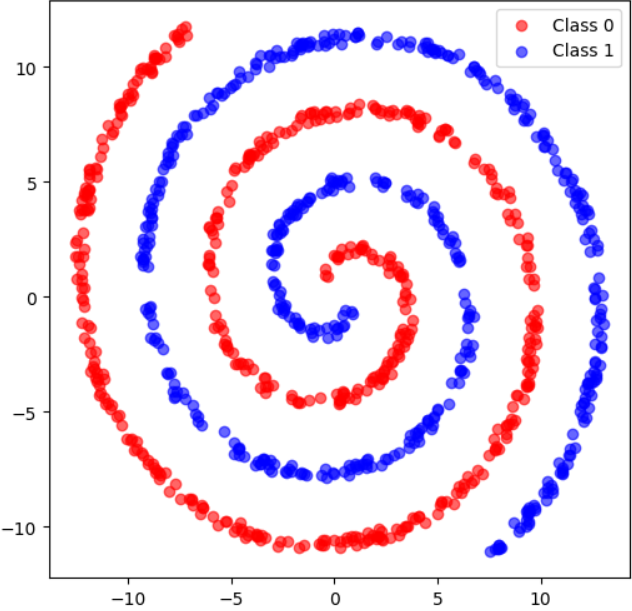
\includegraphics[width=0.23\textwidth]{../Images/OG_Spiral.PNG}%
        \label{fig:og_spiral}
    }
    \hfil
    \subfloat[Normalised Spiral With $\hfill$ Added Noise]{%
        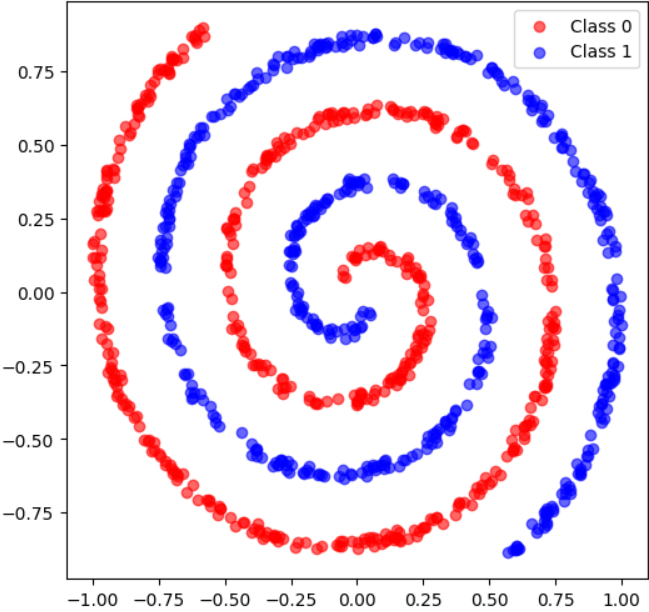
\includegraphics[width=0.23\textwidth]{../Images/Normal_Spiral.PNG}%
        \label{fig:normal_spiral}
    }
    \caption{Randomly Generated Spiral Dataset}
    \label{fig:Spiral}
\end{figure}

Since the dataset has balanced classes, the prediction accuracy serves as the performance
metric used to evaluate the influence of the number of ensemble members and the bag sizes.
A random seed is initialised to ensure reproducibility of the generated dataset.

\subsection{Experimental Setup} \label{section: experimental_setup_emp}

\subsubsection{Obtaining the results}
The grids $[0.4, 0.5, 0.6, 0.7, 0.8]$, $[0.4, 0.5, 0.6, 0.7, 0.8]$ and $[5, 10, 20, 50, 100]$
were used to investigate the influence of the size of the bag, the number of randomly selected features and
the number of ensemble members, respectively, for both the linear and non-linear logistic regression ensembles.
However, the spiral dataset contains only 2 descriptive features and therefore, only the influence
of the bag size and the number of ensemble methods were investigated with their respective grids of
$[0.4, 0.5, 0.6, 0.7, 0.8]$ and $[5, 10, 20, 50, 100]$.

A 5-fold cross-validation was also conducted for each possible combination of the grid values, which is also known as
the grid search technique. For each dataset, the cross validation splits the data up into five datasets, where four
sets were used to construct the model with the associated values of the grids and the set that remains was used as the
test set to evaluate the model performance. This process was repeated 5 times to ensure each subset is used as the test
set once. The utilisation of the 5-fold cross validation technique ensured that the evaluation was fair and consistent
across the entire dataset and the bias that might arise from relying on a single training-test split was reduced.

\subsubsection{Finding the optimal control parameters}
To find the optimal control parameters of each optimisation algorithm for each task, a 5-fold
cross-validation was used, as described above, for each dataset.
A Bayesian optimisation technique efficiently searched the hyperparameter space
to identify the parameters that minimised the average test accuracy error for the banana quality and spiral datasets
and the parameters that minimised the average test F1-score for the breast cancer, ionosphere, and diabetes datasets
across the 5-fold cross validation.

\subsection{Control Parameters} \label{section: control_parameters}

Bayesian optimisation is used to find the optimal control parameter for each dataset,
as described in Section \ref{section: experimental_setup_emp}.
The optimal control parameters used for each linear logistic regression ensemble are represented
in Table \ref{table: LR_control_parameters}.
\begin{table}[h!]
    \caption{Linear Logistic Regression Control Parameters}
    \begin{center}
        \begin{tabular}{|c||c|c|c|}
            \hline
            \textbf{Dataset}&\multicolumn{3}{|c|}{\textbf{Control Parameters}} \\
            % \textbf{Max depth}
            \cline{2-4}
                        & \textbf{\textit{eta}} & \textbf{\textit{epochs}} & \textbf{\textit{patience}}\\
            \hline
            \textbf{\textit{Breast Cancer}} & 0.00239 & 10678 & 6 \\
            \textbf{\textit{Ionosphere}} & 0.00012 & 9809 & 6\\
            \textbf{\textit{Diabetes}} & 0.01121 & 18690 & 9\\
            \textbf{\textit{Banana Quality}}  & 0.00023 & 4338 & 5 \\
            \textbf{\textit{Spiral}} & 0.06708 & 17335 & 7\\
            \hline
        \end{tabular}
    \end{center}
    \label{table: LR_control_parameters}
\end{table}

The optimal control parameters used for each non-linear logistic regression ensemble are represented
in Table \ref{table: NLR_control_parameters}.
\begin{table}[h!]
    \caption{Non-Linear Logistic Regression Control Parameters}
    \begin{center}
        \begin{tabular}{|c||c|c|c|c|c|}
            \hline
            \textbf{Dataset}&\multicolumn{5}{|c|}{\textbf{Control Parameters}} \\
            % \textbf{Max depth}
            \cline{2-6}
                        & \textbf{\textit{eta}} & \textbf{\textit{epochs}} & \textbf{\textit{patience}} & \textbf{\textit{poly}} & \textbf{\textit{\% poly}}\\
            \hline
            \textbf{\textit{Breast Cancer}} & 0.00013 & 3812 & 5 & 3 & 50\\
            \textbf{\textit{Ionosphere}} & 0.0001 & 2797 & 10 & 3 & 70\\
            \textbf{\textit{Diabetes}} & 0.00783 & 1000 & 6 & 3 & 80\\
            \textbf{\textit{Banana Quality}} & 0.01099 & 5054 & 5 & 3 & 80\\
            \textbf{\textit{Spiral}} & 0.00011 & 8755 & 5 & 4 & 60\\
            \hline
        \end{tabular}
    \end{center}
    \label{table: NLR_control_parameters}
\end{table}

\subsection{Statistical Significance and Analysis}

The statistical significance of the results from the the grid search of each dataset for the linear and
non-linear logistic regression ensemble is determined by the evaluation of the accuracy for banana quality and spiral
dataset and the F1-score for the breast cancer, ionosphere and diabetes dataset, by the utilisation of a 5-fold cross validation. 
For each dataset, the Kruskal-Wallis test was used to evaluate the statistical significance of differences among the grid search
results across various parameter combinations, with a significance level of 0.05. Additionally, for each dataset, the
paired t-test was performed to compare the results of the linear and non-linear logistic regression ensemble models,
which assessed the statistical significance between their performance distributions, with a significance level of 0.05.

\section{Research Results} \label{section: Research Results}

This section presents the results of the evaluation of the linear and non-linear logistic regression ensembles across the five
binary classification datasets. Key factors examined include the influence of ensemble size, bag size, and feature subset
size on classification performance.

\subsection{Breast Cancer Dataset}

By use of Bayesian optimisation, the optimal values of the control parameters in the
linear and non-linear logistic regression ensembles are determined as seen in
Section \ref{section: control_parameters}.

A 5-fold cross validation technique is then applied to the grid search of the linear and non-linear logistic regression ensemble models
to investigate the influence of the size of the bag, the number of randomly selected features and
the number of ensemble members as seen in Section \ref{section: experimental_setup_emp}.

\subsubsection{Bag size}

Table \ref{table: BC_bagsize_linear_performance_metrics} presents the mean, standard deviation, minimum and maximum of the
F1-scores from the 5-fold cross-validation of the linear logistic regression ensemble, grouped by each bag size
value in the grid.
\begin{table}[H]
    \caption{Summary Statistics of F1-Scores for Each Bag Size of the Linear Logistic Regression Ensemble on the Breast Cancer Dataset}
    \begin{center}
        \begin{tabular}{|c||c|c|c|c|c|}
            \hline
            \textbf{Bag Size}&\multicolumn{5}{|c|}{\textbf{Summary Statistics}} \\
            % \textbf{Max depth}
            \cline{2-6}
                       &\textbf{\textit{count}} & \textbf{\textit{mean}} & \textbf{\textit{std}} & \textbf{\textit{min}} & \textbf{\textit{max}}\\
            \hline
            \textbf{\textit{0.4}} & 125 & 97.66 & 0.0103 & 94.89 & 99.35\\
            \textbf{\textit{0.5}} & 125 & 97.47 & 0.0099 & 94.96 & 99.35\\
            \textbf{\textit{0.6}} & 125 & 97.88 & 0.0097 & 94.03 & 99.35\\
            \textbf{\textit{0.7}} & 125 & 97.85 & 0.0099 & 95.65 & 99.35\\
            \textbf{\textit{0.8}} & 125 & 97.91 & 0.0096 & 95.83 & 99.35\\
            \hline
        \end{tabular}
    \end{center}
    \label{table: BC_bagsize_linear_performance_metrics}
\end{table}
The Kruskal-Wallis test returned a p-value of 0.3895 between the scores of the linear logistic regression ensemble model,
which means there is no significant difference between the scores. Therefore, the bag size has a minimal effect on the
performance of the linear logistic regression ensemble on the breast cancer dataset.

Table \ref{table: BC_bagsize_nonlinear_performance_metrics} presents the mean, standard deviation, minimum and maximum of the
F1-scores from the 5-fold cross-validation of the non-linear logistic regression ensemble, grouped by each bag size
value in the grid.
\begin{table}[H]
    \caption{Summary Statistics of F1-Scores for Each Bag Size of the Non-Linear Logistic Regression Ensemble on the Breast Cancer Dataset}
    \begin{center}
        \begin{tabular}{|c||c|c|c|c|c|}
            \hline
            \textbf{Bag Size}&\multicolumn{5}{|c|}{\textbf{Summary Statistics}} \\
            % \textbf{Max depth}
            \cline{2-6}
                                &\textbf{\textit{count}} & \textbf{\textit{mean}} & \textbf{\textit{std}} & \textbf{\textit{min}} & \textbf{\textit{max}}\\
            \hline
            \textbf{\textit{0.4}} & 125 & 97.37 & 0.0100 & 94.52 & 99.35 \\
            \textbf{\textit{0.5}} & 125 & 97.69 & 0.0097 & 95.59 & 99.35 \\
            \textbf{\textit{0.6}} & 125 & 97.83 & 0.0088 & 95.83 & 99.35 \\
            \textbf{\textit{0.7}} & 125 & 97.81 & 0.0100 & 94.96 & 1 \\
            \textbf{\textit{0.8}} & 125 & 97.92 & 0.0105 & 95.59 & 1 \\
            \hline
        \end{tabular}
    \end{center}
    \label{table: BC_bagsize_nonlinear_performance_metrics}
\end{table}
The Kruskal-Wallis test returned a p-value of 0.004 between the scores of the non-linear logistic regression ensemble model,
which means there is a significant difference between the scores. Therefore, the bag size has a notable effect on the
performance of the non-linear logistic regression ensemble on the breast cancer dataset.

The mean F1-scores obtained from each value of bag size in the grid from both the linear and non-linear
logistic regression ensemble models is presented in Figure \ref{fig:BC_bag_comparison}.
\begin{figure}[H]
    \centerline{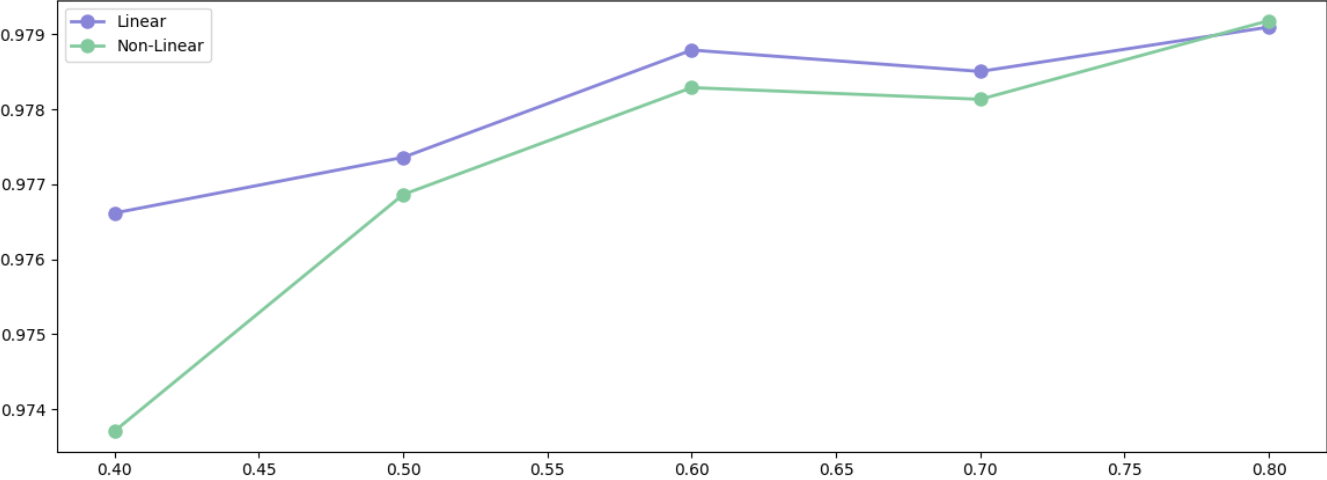
\includegraphics[scale=0.26]{../Images/BC_bag.PNG}}
    \caption{Comparison of mean F1-score across the bag size grid when the breast cancer dataset is classified by use of 5-fold cross-validation.}
    \label{fig:BC_bag_comparison}
\end{figure}
From figure \ref{fig:BC_bag_comparison} it is seen that the linear logistic regression ensemble model performs slightly better
at smaller bag sizes and maintains a more stable performance across the range. The non-linear logistic regression ensemble model
starts with lower performance at small bag sizes but catches up to the linear model at larger bag sizes,
at a bag size of 0.80 with an average F1-score of approximately 0.979 the models converge. The differences between
the two models are quite small, with average F1-scores which only varys between about 0.974 and 0.979.

The paired t-test between the two models returned a p-value of 0.1880, which indicates there is no significant difference
between the average F1-scores of the linear and non-linear logistic regression ensembles based on the breast cancer dataset.

The linear logistic regression model performs better for smaller bag sizes and the models performs similarly on larger
bag sizes. Therefore the linear logistic ensemble model performs best on the breast cancer dataset when the bag size is considered.

\subsubsection{Number of features}

Table \ref{table: BC_features_linear_performance_metrics} presents the mean, standard deviation, minimum and maximum of the
F1-scores from the 5-fold cross-validation of the linear logistic regression ensemble, grouped by each number of randomly selected
features value in the grid.
\begin{table}[H]
    \caption{Summary Statistics of F1-Scores for Each Number of Features of the Linear Logistic Regression Ensemble on the Breast Cancer Dataset}
    \begin{center}
        \begin{tabular}{|c||c|c|c|c|c|}
            \hline
            \textbf{Number of Featurs}&\multicolumn{5}{|c|}{\textbf{Summary Statistics}} \\
            % \textbf{Max depth}
            \cline{2-6}
                       &\textbf{\textit{count}} & \textbf{\textit{mean}} & \textbf{\textit{std}} & \textbf{\textit{min}} & \textbf{\textit{max}}\\
            \hline
            \textbf{\textit{0.4}} & 125 & 97.62 & 0.0099 & 94.03 & 99.35 \\
            \textbf{\textit{0.5}} & 125 & 97.70 & 0.0111 & 94.89 & 99.35 \\
            \textbf{\textit{0.6}} & 125 & 97.90 & 0.0095 & 95.71 & 99.35 \\
            \textbf{\textit{0.7}} & 125 & 97.89 & 0.0096 & 95.83 & 99.35 \\
            \textbf{\textit{0.8}} & 125 & 97.92 & 0.0090 & 95.83 & 99.35 \\
            \hline
        \end{tabular}
    \end{center}
    \label{table: BC_features_linear_performance_metrics}
\end{table}
The Kruskal-Wallis test returned a p-value of 0.1813 between the scores of the linear logistic regression ensemble model,
which means there is no significant difference between the scores. Therefore, the number of randomly selected
features has a minimal effect on the performance of the linear logistic regression ensemble on the breast cancer dataset.

Table \ref{table: BC_feature_nonlinear_performance_metrics} presents the mean, standard deviation, minimum and maximum of the
F1-scores from the 5-fold cross-validation of the non-linear logistic regression ensemble, grouped by each number of randomly selected
features value in the grid.
\begin{table}[H]
    \caption{Summary Statistics of F1-Scores for Each Number of Features of the Non-Linear Logistic Regression Ensemble on the Breast Cancer Dataset}
    \begin{center}
        \begin{tabular}{|c||c|c|c|c|c|}
            \hline
            \textbf{Number of Features}&\multicolumn{5}{|c|}{\textbf{Summary Statistics}} \\
            % \textbf{Max depth}
            \cline{2-6}
                                &\textbf{\textit{count}} & \textbf{\textit{mean}} & \textbf{\textit{std}} & \textbf{\textit{min}} & \textbf{\textit{max}}\\
            \hline
            \textbf{\textit{0.4}} & 125 & 97.28 & 0.0099 & 94.52 & 99.35 \\
            \textbf{\textit{0.5}} & 125 & 97.59 & 0.0093 & 94.89 & 99.35 \\
            \textbf{\textit{0.6}} & 125 & 97.77 & 0.0092 & 94.96 & 1 \\
            \textbf{\textit{0.7}} & 125 & 97.87 & 0.0097 & 94.89 & 1 \\
            \textbf{\textit{0.8}} & 125 & 98.11 & 0.0099 & 95.77 & 1 \\
            \hline
        \end{tabular}
    \end{center}
    \label{table: BC_feature_nonlinear_performance_metrics}
\end{table}
The Kruskal-Wallis test returned a p-value of 0 between the scores of the non-linear logistic regression ensemble model,
which means there is a significant difference between the scores. Therefore, the number of randomly selected
features has a notable effect on the performance of the non-linear logistic regression ensemble on the breast cancer dataset.

The mean F1-scores obtained from each value of number of randomly selected features in the grid from both the linear and non-linear
logistic regression ensemble models is presented in Figure \ref{fig:BC_features_comparison}.
\begin{figure}[H]
    \centerline{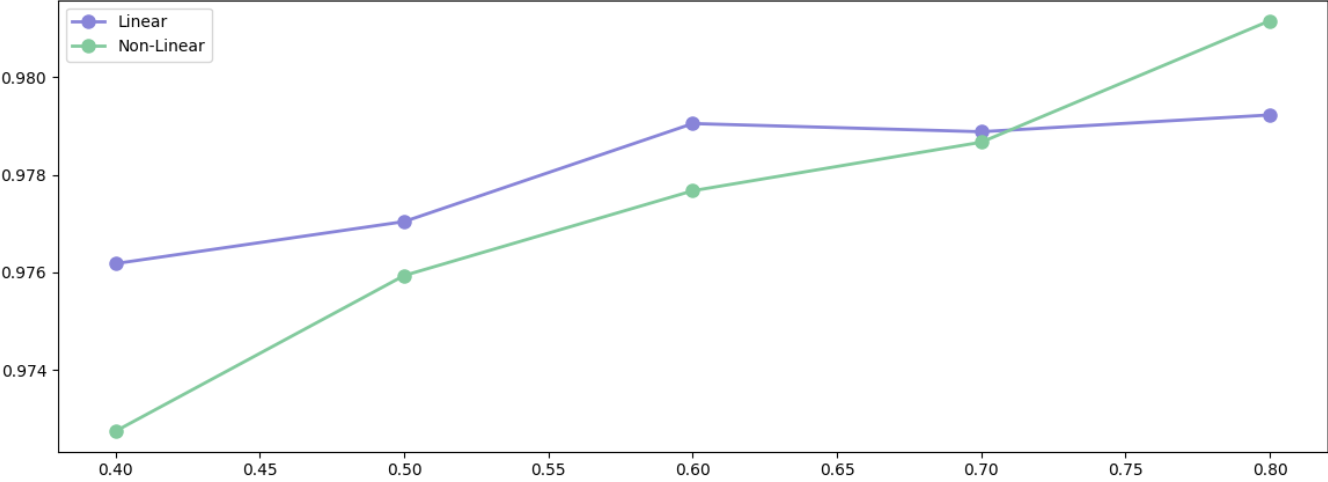
\includegraphics[scale=0.26]{../Images/BC_features.PNG}}
    \caption{Comparison of mean F1-score across the number of randomly selected features grid when the breast cancer dataset is classified by use of 5-fold cross-validation.}
    \label{fig:BC_features_comparison}
\end{figure}
From figure \ref{fig:BC_features_comparison} it is seen that the linear logistic regression ensemble model performs slightly better
at less number of features and maintains a more stable performance across the range. The non-linear logistic regression ensemble model
starts with lower performance at less number of features but catches up to the linear model at more number of features,
at a number of features of 0.70 with an average F1-score of approximately 0.978 the models converge. The non-linear
logistic regression ensemble model then performs much better than the linear logistic regression ensemble model at a number
of features of 0.8. The differences between the two models are quite small, with average F1-scores which only varys between about
0.972 and 0.982.

The paired t-test between the two models returned a p-value of 0.3895, which indicates there is no significant difference
between the average F1-scores of the linear and non-linear logistic regression ensembles based on the breast cancer dataset.

For less number of features, the linear logistic regression performs best and for more number of
features, the non-linear logistic regression performs best. Therefore, there is no clear ensemble model
that performs best on the breast cancer dataset when the number of features are considered.

\subsubsection{Number of ensemble members}

Table \ref{table: BC_member_linear_performance_metrics} presents the mean, standard deviation, minimum and maximum of the
F1-scores from the 5-fold cross-validation of the linear logistic regression ensemble, grouped by each number of ensemble members
value in the grid.
\begin{table}[H]
    \caption{Summary Statistics of F1-Scores for Each Number of Ensemble Members of the Linear Logistic Regression Ensemble on the Breast Cancer Dataset}
    \begin{center}
        \begin{tabular}{|c||c|c|c|c|c|}
            \hline
            \textbf{Number of Featurs}&\multicolumn{5}{|c|}{\textbf{Summary Statistics}} \\
            % \textbf{Max depth}
            \cline{2-6}
                       &\textbf{\textit{count}} & \textbf{\textit{mean}} & \textbf{\textit{std}} & \textbf{\textit{min}} & \textbf{\textit{max}}\\
            \hline
            \textbf{\textit{5}} & 125 & 97.66 & 0.0106 & 94.03 & 99.35 \\
            \textbf{\textit{10}} & 125 & 97.74 & 0.0100 & 95.65 & 99.35 \\
            \textbf{\textit{20}} & 125 & 97.88 & 0.0094 & 95.83 & 99.35 \\
            \textbf{\textit{50}} & 125 & 97.86 & 0.0101 & 95.65 & 99.35 \\
            \textbf{\textit{100}} & 125 & 97.90 & 0.0093 & 95.83 & 99.35 \\
            \hline
        \end{tabular}
    \end{center}
    \label{table: BC_member_linear_performance_metrics}
\end{table}
The Kruskal-Wallis test returned a p-value of 0.4252 between the scores of the linear logistic regression ensemble model,
which means there is no significant difference between the scores. Therefore, the number of ensemble members
has a minimal effect on the performance of the linear logistic regression ensemble on the breast cancer dataset.

Table \ref{table: BC_member_nonlinear_performance_metrics} presents the mean, standard deviation, minimum and maximum of the
F1-scores from the 5-fold cross-validation of the non-linear logistic regression ensemble, grouped by each number of ensemble members
value in the grid.
\begin{table}[H]
    \caption{Summary Statistics of F1-Scores for Each Number of Ensemble Members of the Non-Linear Logistic Regression Ensemble on the Breast Cancer Dataset}
    \begin{center}
        \begin{tabular}{|c||c|c|c|c|c|}
            \hline
            \textbf{Number of Features}&\multicolumn{5}{|c|}{\textbf{Summary Statistics}} \\
            % \textbf{Max depth}
            \cline{2-6}
                                &\textbf{\textit{count}} & \textbf{\textit{mean}} & \textbf{\textit{std}} & \textbf{\textit{min}} & \textbf{\textit{max}}\\
            \hline
            \textbf{\textit{5}} & 125 & 97.35 & 0.0125 & 94.52 & 1 \\
            \textbf{\textit{10}} & 125 & 97.62 & 0.0098 & 95.59 & 1 \\
            \textbf{\textit{20}} & 125 & 97.80 & 0.0091 & 95.65 & 99.35 \\
            \textbf{\textit{50}} & 125 & 97.90 & 0.0085 & 96.35 & 99.35 \\
            \textbf{\textit{100}} & 125 & 97.94 & 0.0084 & 96.35 & 99.35 \\
            \hline
        \end{tabular}
    \end{center}
    \label{table: BC_member_nonlinear_performance_metrics}
\end{table}
The Kruskal-Wallis test returned a p-value of 0.0003 between the scores of the non-linear logistic regression ensemble model,
which means there is a significant difference between the scores. Therefore, the number of ensemble members
has a notable effect on the performance of the non-linear logistic regression ensemble on the breast cancer dataset.

The mean F1-scores obtained from each value of number of ensemble members in the grid from both the linear and non-linear
logistic regression ensemble models is presented in Figure \ref{fig:BC_member_comparison}.
\begin{figure}[H]
    \centerline{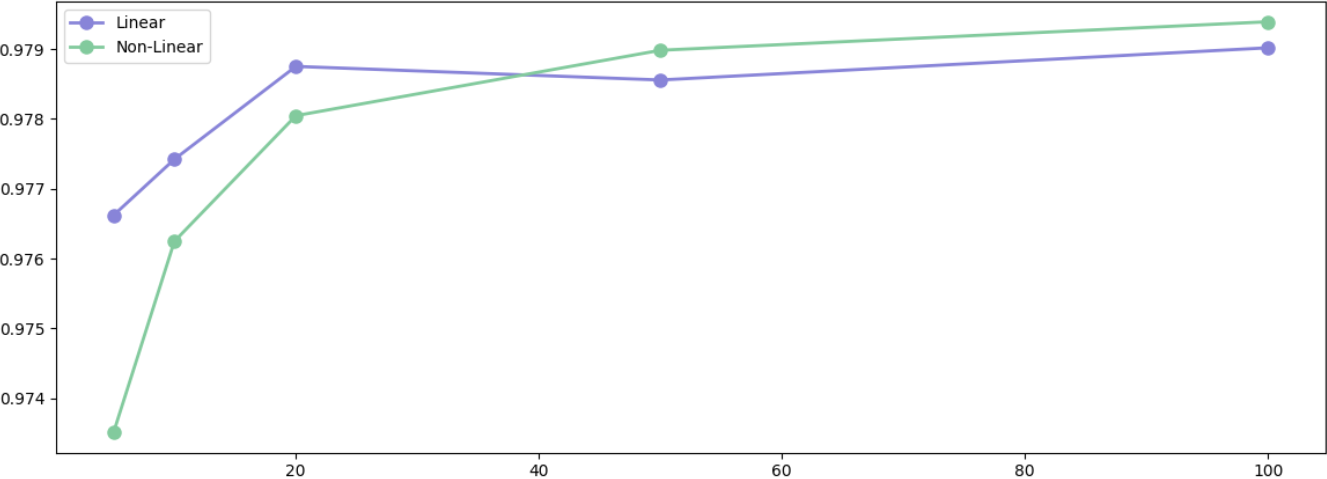
\includegraphics[scale=0.26]{../Images/BC_members.PNG}}
    \caption{Comparison of mean F1-score across the number of ensemble members grid when the breast cancer dataset is classified by use of 5-fold cross-validation.}
    \label{fig:BC_member_comparison}
\end{figure}
From figure \ref{fig:BC_member_comparison} it is seen that the linear logistic regression ensemble model performs slightly better
at less ensemble members and maintains a more stable performance across the range. The non-linear logistic regression ensemble model
starts with lower performance at less ensemble members but catches up to the linear model at more ensemble members,
at a number of ensemble members of 40 with an average F1-score of approximately 0.9785 the models converge. The non-linear
logistic regression ensemble model then performs much better than the linear logistic regression ensemble model at a number
of ensemble members of 50 and higher. The differences between the two models are quite small, with average F1-scores which only
varys between about 0.973 and 0.98.

The paired t-test between the two models returned a p-value of 0.2643, which indicates there is no significant difference
between the average F1-scores of the linear and non-linear logistic regression ensembles based on the breast cancer dataset.

For a lower number of ensemble members, the linear logistic regression performs best and for a
higher number of ensemble members, the non-linear logistic regression performs best. Therefore, there is
no clear ensemble model that performs best on the breast cancer dataset when the number of ensemble members
are considered.

\subsection{Ionosphere Dataset}

By use of Bayesian optimisation, the optimal values of the control parameters in the
linear and non-linear logistic regression ensembles are determined as seen in
Section \ref{section: control_parameters}.

A 5-fold cross validation technique is then applied to the grid search of the linear and non-linear logistic regression ensemble models
to investigate the influence of the size of the bag, the number of randomly selected features and
the number of ensemble members as seen in Section \ref{section: experimental_setup_emp}.

\subsubsection{Bag size}

Table \ref{table: I_bagsize_linear_performance_metrics} presents the mean, standard deviation, minimum and maximum of the
F1-scores from the 5-fold cross-validation of the linear logistic regression ensemble, grouped by each bag size
value in the grid.
\begin{table}[H]
    \caption{Summary Statistics of F1-Scores for Each Bag Size of the Linear Logistic Regression Ensemble on the Ionosphere Dataset}
    \begin{center}
        \begin{tabular}{|c||c|c|c|c|c|}
            \hline
            \textbf{Bag Size}&\multicolumn{5}{|c|}{\textbf{Summary Statistics}} \\
            % \textbf{Max depth}
            \cline{2-6}
                       &\textbf{\textit{count}} & \textbf{\textit{mean}} & \textbf{\textit{std}} & \textbf{\textit{min}} & \textbf{\textit{max}}\\
            \hline
            \textbf{\textit{0.4}} & 125 & 88.22 & 0.0214 & 84.21 & 93.20 \\
            \textbf{\textit{0.5}} & 125 & 88.58 & 0.0180 & 85.11 & 92.31 \\
            \textbf{\textit{0.6}} & 125 & 88.39 & 0.0191 & 84.11 & 92.16 \\
            \textbf{\textit{0.7}} & 125 & 88.80 & 0.0164 & 84.21 & 92.16 \\
            \textbf{\textit{0.8}} & 125 & 88.88 & 0.0172 & 85.11 & 92.16 \\
            \hline
        \end{tabular}
    \end{center}
    \label{table: I_bagsize_linear_performance_metrics}
\end{table}
The Kruskal-Wallis test returned a p-value of 0.0078 between the scores of the linear logistic regression ensemble model,
which means there is a significant difference between the scores. Therefore, the bag size has a notable effect on the
performance of the linear logistic regression ensemble on the ionosphere dataset.

Table \ref{table: I_bagsize_nonlinear_performance_metrics} presents the mean, standard deviation, minimum and maximum of the
F1-scores from the 5-fold cross-validation of the non-linear logistic regression ensemble, grouped by each bag size
value in the grid.
\begin{table}[H]
    \caption{Summary Statistics of F1-Scores for Each Bag Size of the Non-Linear Logistic Regression Ensemble on the Ionosphere Dataset}
    \begin{center}
        \begin{tabular}{|c||c|c|c|c|c|}
            \hline
            \textbf{Bag Size}&\multicolumn{5}{|c|}{\textbf{Summary Statistics}} \\
            % \textbf{Max depth}
            \cline{2-6}
                                &\textbf{\textit{count}} & \textbf{\textit{mean}} & \textbf{\textit{std}} & \textbf{\textit{min}} & \textbf{\textit{max}}\\
            \hline
            \textbf{\textit{0.4}} & 125 & 91.72 & 0.0221 & 86.87 & 95.65 \\
            \textbf{\textit{0.5}} & 125 & 92.40 & 0.0220 & 83.33 & 96.00 \\
            \textbf{\textit{0.6}} & 125 & 92.88 & 0.0209 & 86.00 & 96.00 \\
            \textbf{\textit{0.7}} & 125 & 93.43 & 0.0213 & 88.66 & 96.70 \\
            \textbf{\textit{0.8}} & 125 & 93.63 & 0.0184 & 88.89 & 96.70 \\
            \hline
        \end{tabular}
    \end{center}
    \label{table: I_bagsize_nonlinear_performance_metrics}
\end{table}
The Kruskal-Wallis test returned a p-value of 0 between the scores of the non-linear logistic regression ensemble model,
which means there is a significant difference between the scores. Therefore, the bag size has a notable effect on the
performance of the non-linear logistic regression ensemble on the ionosphere dataset.

The mean F1-scores obtained from each value of bag size in the grid from both the linear and non-linear
logistic regression ensemble models is presented in Figure \ref{fig:I_bag_comparison}.
\begin{figure}[H]
    \centerline{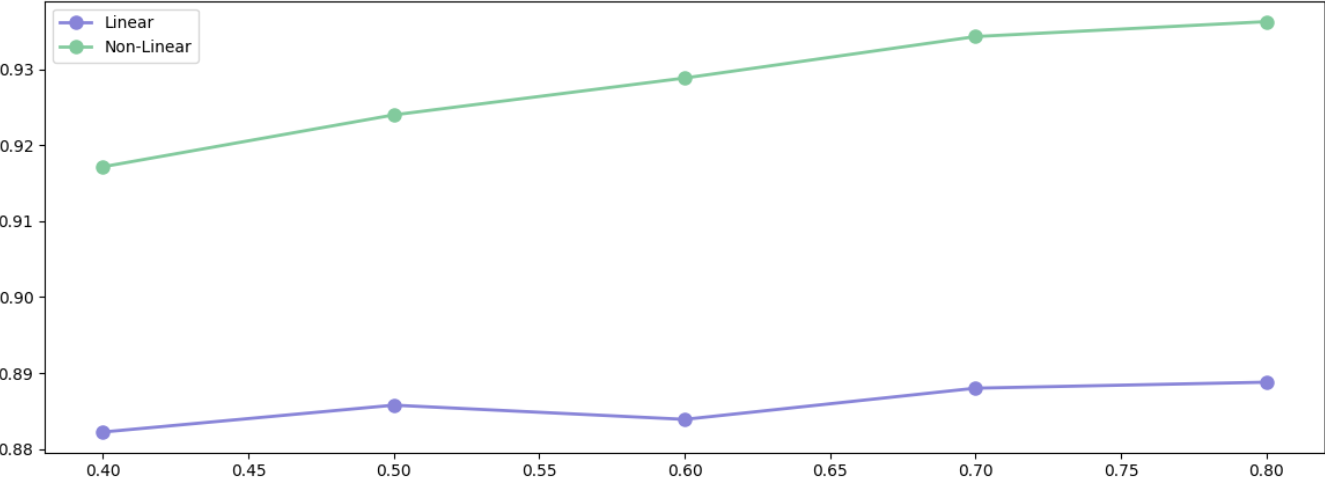
\includegraphics[scale=0.26]{../Images/I_bag.PNG}}
    \caption{Comparison of mean F1-score across the bag size grid when the ionosphere dataset is classified by use of 5-fold cross-validation.}
    \label{fig:I_bag_comparison}
\end{figure}
The optimal bag size for both the linear and non-linear logistic regression ensemble models for the ionosphere dataset is 0.8, which
indicates that the models performs better when constructed on more observations.

The paired t-test between the two models returned a p-value of 0.0001, which indicates there is a significant difference
between the average F1-scores of the linear and non-linear logistic regression ensembles based on the ionosphere dataset.

From figure \ref{fig:I_bag_comparison} it is seen that the non-linear logistic regression ensemble performs best across
all different bag sizes. Therefore the non-linear logistic ensemble model performs best on the ionosphere dataset when the
bag size is considered.

\subsubsection{Number of features}

Table \ref{table: I_features_linear_performance_metrics} presents the mean, standard deviation, minimum and maximum of the
F1-scores from the 5-fold cross-validation of the linear logistic regression ensemble, grouped by each number of randomly selected
features value in the grid.
\begin{table}[H]
    \caption{Summary Statistics of F1-Scores for Each Number of Features of the Linear Logistic Regression Ensemble on the Ionosphere Dataset}
    \begin{center}
        \begin{tabular}{|c||c|c|c|c|c|}
            \hline
            \textbf{Number of Featurs}&\multicolumn{5}{|c|}{\textbf{Summary Statistics}} \\
            % \textbf{Max depth}
            \cline{2-6}
                       &\textbf{\textit{count}} & \textbf{\textit{mean}} & \textbf{\textit{std}} & \textbf{\textit{min}} & \textbf{\textit{max}}\\
            \hline
            \textbf{\textit{0.4}} & 125 & 88.31 & 0.0194 & 84.21 & 92.31 \\
            \textbf{\textit{0.5}} & 125 & 88.29 & 0.0195 & 84.11 & 92.31 \\
            \textbf{\textit{0.6}} & 125 & 88.62 & 0.0179 & 85.11 & 92.31 \\
            \textbf{\textit{0.7}} & 125 & 88.76 & 0.0181 & 85.11 & 93.20 \\
            \textbf{\textit{0.8}} & 125 & 88.89 & 0.0176 & 85.11 & 93.20 \\
            \hline
        \end{tabular}
    \end{center}
    \label{table: I_features_linear_performance_metrics}
\end{table}
The Kruskal-Wallis test returned a p-value of 0.0118 between the scores of the linear logistic regression ensemble model,
which means there is a significant difference between the scores. Therefore, the number of randomly selected
features has a notable effect on the performance of the linear logistic regression ensemble on the ionosphere dataset.

Table \ref{table: I_feature_nonlinear_performance_metrics} presents the mean, standard deviation, minimum and maximum of the
F1-scores from the 5-fold cross-validation of the non-linear logistic regression ensemble, grouped by each number of randomly selected
features value in the grid.
\begin{table}[H]
    \caption{Summary Statistics of F1-Scores for Each Number of Features of the Non-Linear Logistic Regression Ensemble on the Ionosphere Dataset}
    \begin{center}
        \begin{tabular}{|c||c|c|c|c|c|}
            \hline
            \textbf{Number of Features}&\multicolumn{5}{|c|}{\textbf{Summary Statistics}} \\
            % \textbf{Max depth}
            \cline{2-6}
                                &\textbf{\textit{count}} & \textbf{\textit{mean}} & \textbf{\textit{std}} & \textbf{\textit{min}} & \textbf{\textit{max}}\\
            \hline
            \textbf{\textit{0.4}} & 125 & 92.15 & 0.0261 & 83.33 & 96 \\
            \textbf{\textit{0.5}} & 125 & 92.94 & 0.0197 & 87.91 & 96.7 \\
            \textbf{\textit{0.6}} & 125 & 93.09 & 0.0202 & 88.89 & 96.7 \\
            \textbf{\textit{0.7}} & 125 & 93.03 & 0.0208 & 88.89 & 96.7 \\
            \textbf{\textit{0.8}} & 125 & 92.84 & 0.0217 & 87.91 & 96.7 \\
            \hline
        \end{tabular}
    \end{center}
    \label{table: I_feature_nonlinear_performance_metrics}
\end{table}
The Kruskal-Wallis test returned a p-value of 0.0166 between the scores of the non-linear logistic regression ensemble model,
which means there is a significant difference between the scores. Therefore, the number of randomly selected
features has a notable effect on the performance of the non-linear logistic regression ensemble on the ionosphere dataset.

The mean F1-scores obtained from each value of number of randomly selected features in the grid from both the linear and non-linear
logistic regression ensemble models is presented in Figure \ref{fig:I_features_comparison}.
\begin{figure}[H]
    \centerline{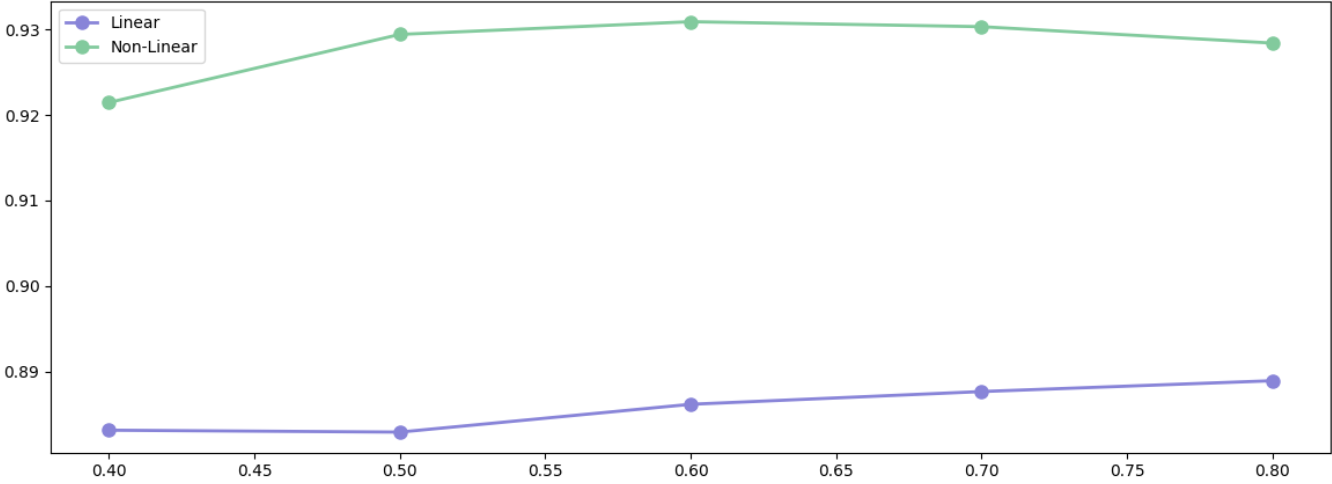
\includegraphics[scale=0.26]{../Images/I_features.PNG}}
    \caption{Comparison of mean F1-score across the number of randomly selected features grid when the ionosphere dataset is classified by use of 5-fold cross-validation.}
    \label{fig:I_features_comparison}
\end{figure}
The linear logistic regression ensemble model has a slight increase in F1-score on the ionosphere dataset when the number of features are increased
and the F1-score of the non-linear logistic regression ensemble model remains stable with values of 0.5 to 0.7 and decreases when 80\%
of the features are included when the model is constructed. Therefore the optimal value of features to use is 0.5. 

The paired t-test between the two models returned a p-value of 0, which indicates there is a significant difference
between the average F1-scores of the linear and non-linear logistic regression ensembles based on the ionosphere dataset.

From figure \ref{fig:I_features_comparison} it is seen that the non-linear logistic regression ensemble performs best across
all different number of features. Therefore the non-linear logistic ensemble model performs best on the ionosphere dataset when the
number of features is considered.

\subsubsection{Number of ensemble members}

Table \ref{table: I_member_linear_performance_metrics} presents the mean, standard deviation, minimum and maximum of the
F1-scores from the 5-fold cross-validation of the linear logistic regression ensemble, grouped by each number of ensemble members
value in the grid.
\begin{table}[H]
    \caption{Summary Statistics of F1-Scores for Each Number of Ensemble Members of the Linear Logistic Regression Ensemble on the Ionosphere Dataset}
    \begin{center}
        \begin{tabular}{|c||c|c|c|c|c|}
            \hline
            \textbf{Number of Featurs}&\multicolumn{5}{|c|}{\textbf{Summary Statistics}} \\
            % \textbf{Max depth}
            \cline{2-6}
                       &\textbf{\textit{count}} & \textbf{\textit{mean}} & \textbf{\textit{std}} & \textbf{\textit{min}} & \textbf{\textit{max}}\\
            \hline
            \textbf{\textit{5}}   & 125 & 88.34 & 0.0205 & 84.21 & 92.31 \\
            \textbf{\textit{10}}  & 125 & 88.57 & 0.0179 & 84.11 & 92.31 \\
            \textbf{\textit{20}}  & 125 & 88.50 & 0.0182 & 84.21 & 92.16 \\
            \textbf{\textit{50}}  & 125 & 88.70 & 0.0181 & 86.00 & 93.20 \\
            \textbf{\textit{100}} & 125 & 88.75 & 0.0181 & 86.00 & 92.31 \\
            \hline
        \end{tabular}
    \end{center}
    \label{table: I_member_linear_performance_metrics}
\end{table}
The Kruskal-Wallis test returned a p-value of 0.4025 between the scores of the linear logistic regression ensemble model,
which means there is no significant difference between the scores. Therefore, the number of ensemble members
has a minimal effect on the performance of the linear logistic regression ensemble on the ionosphere dataset.

Table \ref{table: I_member_nonlinear_performance_metrics} presents the mean, standard deviation, minimum and maximum of the
F1-scores from the 5-fold cross-validation of the non-linear logistic regression ensemble, grouped by each number of ensemble members
value in the grid.
\begin{table}[H]
    \caption{Summary Statistics of F1-Scores for Each Number of Ensemble Members of the Non-Linear Logistic Regression Ensemble on the Ionosphere Dataset}
    \begin{center}
        \begin{tabular}{|c||c|c|c|c|c|}
            \hline
            \textbf{Number of Features}&\multicolumn{5}{|c|}{\textbf{Summary Statistics}} \\
            % \textbf{Max depth}
            \cline{2-6}
                                &\textbf{\textit{count}} & \textbf{\textit{mean}} & \textbf{\textit{std}} & \textbf{\textit{min}} & \textbf{\textit{max}}\\
            \hline
            \textbf{\textit{5}}   & 125 & 91.92 & 0.0247 & 83.33 & 96.7 \\
            \textbf{\textit{10}}  & 125 & 92.75 & 0.0212 & 86.87 & 96.7 \\
            \textbf{\textit{20}}  & 125 & 92.95 & 0.0210 & 86.87 & 96.7 \\
            \textbf{\textit{50}}  & 125 & 93.21 & 0.0201 & 87.76 & 96.7 \\
            \textbf{\textit{100}} & 125 & 93.23 & 0.0206 & 86.87 & 96.7 \\
            \hline
        \end{tabular}
    \end{center}
    \label{table: I_member_nonlinear_performance_metrics}
\end{table}
The Kruskal-Wallis test returned a p-value of 0.0001 between the scores of the non-linear logistic regression ensemble model,
which means there is a significant difference between the scores. Therefore, the number of ensemble members
has a notable effect on the performance of the non-linear logistic regression ensemble on the ionosphere dataset.

The mean F1-scores obtained from each value of number of ensemble members in the grid from both the linear and non-linear
logistic regression ensemble models is presented in Figure \ref{fig:I_member_comparison}.
\begin{figure}[H]
    \centerline{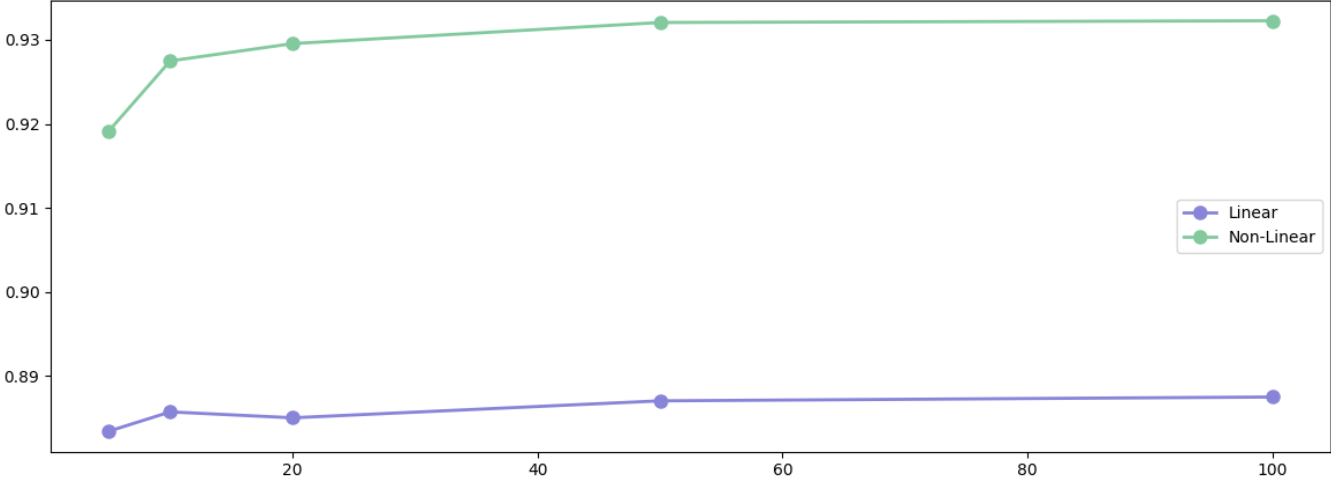
\includegraphics[scale=0.26]{../Images/I_members.PNG}}
    \caption{Comparison of mean F1-score across the number of ensemble members grid when the ionosphere dataset is classified by use of 5-fold cross-validation.}
    \label{fig:I_member_comparison}
\end{figure}
The F1-score for both of the linear and logistic regression ensemble models converges after 20 members in the ensemble. Therefore,
the optimal number of members to use in the linear and logistic regression ensemble models are 10 and 20 respectively.

The paired t-test between the two models returned a p-value of 0, which indicates there is a significant difference
between the average F1-scores of the linear and non-linear logistic regression ensembles based on the ionosphere dataset.

From figure \ref{fig:I_member_comparison} it is seen that the non-linear logistic regression ensemble performs best across
all different number of ensemble members. Therefore the non-linear logistic ensemble model performs best on the ionosphere dataset when the
number of ensemble members is considered.

\subsection{Diabetes Dataset}

By use of Bayesian optimisation, the optimal values of the control parameters in the
linear and non-linear logistic regression ensembles are determined as seen in
Section \ref{section: control_parameters}.

A 5-fold cross validation technique is then applied to the grid search of the linear and non-linear logistic regression ensemble models
to investigate the influence of the size of the bag, the number of randomly selected features and
the number of ensemble members as seen in Section \ref{section: experimental_setup_emp}.

\subsubsection{Bag size}

Table \ref{table: D_bagsize_linear_performance_metrics} presents the mean, standard deviation, minimum and maximum of the
F1-scores from the 5-fold cross-validation of the linear logistic regression ensemble, grouped by each bag size
value in the grid.
\begin{table}[H]
    \caption{Summary Statistics of F1-Scores for Each Bag Size of the Linear Logistic Regression Ensemble on the Diabetes Dataset}
    \begin{center}
        \begin{tabular}{|c||c|c|c|c|c|}
            \hline
            \textbf{Bag Size}&\multicolumn{5}{|c|}{\textbf{Summary Statistics}} \\
            % \textbf{Max depth}
            \cline{2-6}
                       &\textbf{\textit{count}} & \textbf{\textit{mean}} & \textbf{\textit{std}} & \textbf{\textit{min}} & \textbf{\textit{max}}\\
            \hline
            \textbf{\textit{0.4}} & 125 & 90.57 & 0.0225 & 85.78 & 94.05 \\
            \textbf{\textit{0.5}} & 125 & 90.73 & 0.0207 & 86.05 & 93.47 \\
            \textbf{\textit{0.6}} & 125 & 90.60 & 0.0237 & 84.21 & 94.05 \\
            \textbf{\textit{0.7}} & 125 & 90.97 & 0.0205 & 86.51 & 94.05 \\
            \textbf{\textit{0.8}} & 125 & 89.90 & 0.0246 & 82.96 & 93.25 \\
            \hline
        \end{tabular}
    \end{center}
    \label{table: D_bagsize_linear_performance_metrics}
\end{table}
The Kruskal-Wallis test returned a p-value of 0.0032 between the scores of the linear logistic regression ensemble model,
which means there is a significant difference between the scores. Therefore, the bag size has a notable effect on the
performance of the linear logistic regression ensemble on the diabetes dataset.

Table \ref{table: D_bagsize_nonlinear_performance_metrics} presents the mean, standard deviation, minimum and maximum of the
F1-scores from the 5-fold cross-validation of the non-linear logistic regression ensemble, grouped by each bag size
value in the grid.
\begin{table}[H]
    \caption{Summary Statistics of F1-Scores for Each Bag Size of the Non-Linear Logistic Regression Ensemble on the Diabetes Dataset}
    \begin{center}
        \begin{tabular}{|c||c|c|c|c|c|}
            \hline
            \textbf{Bag Size}&\multicolumn{5}{|c|}{\textbf{Summary Statistics}} \\
            % \textbf{Max depth}
            \cline{2-6}
                                &\textbf{\textit{count}} & \textbf{\textit{mean}} & \textbf{\textit{std}} & \textbf{\textit{min}} & \textbf{\textit{max}}\\
            \hline
            \textbf{\textit{0.4}} & 125 & 90.94 & 0.0211 & 85.25 & 93.48 \\
            \textbf{\textit{0.5}} & 125 & 91.39 & 0.0202 & 86.45 & 93.70 \\
            \textbf{\textit{0.6}} & 125 & 91.10 & 0.0213 & 84.63 & 93.48 \\
            \textbf{\textit{0.7}} & 125 & 91.27 & 0.0202 & 86.12 & 93.90 \\
            \textbf{\textit{0.8}} & 125 & 90.78 & 0.0210 & 86.33 & 94.00 \\
            \hline
        \end{tabular}
    \end{center}
    \label{table: D_bagsize_nonlinear_performance_metrics}
\end{table}
The Kruskal-Wallis test returned a p-value of 0.0154 between the scores of the non-linear logistic regression ensemble model,
which means there is a significant difference between the scores. Therefore, the bag size has a notable effect on the
performance of the non-linear logistic regression ensemble on the diabetes dataset.

The mean F1-scores obtained from each value of bag size in the grid from both the linear and non-linear
logistic regression ensemble models is presented in Figure \ref{fig:D_bag_comparison}.
\begin{figure}[H]
    \centerline{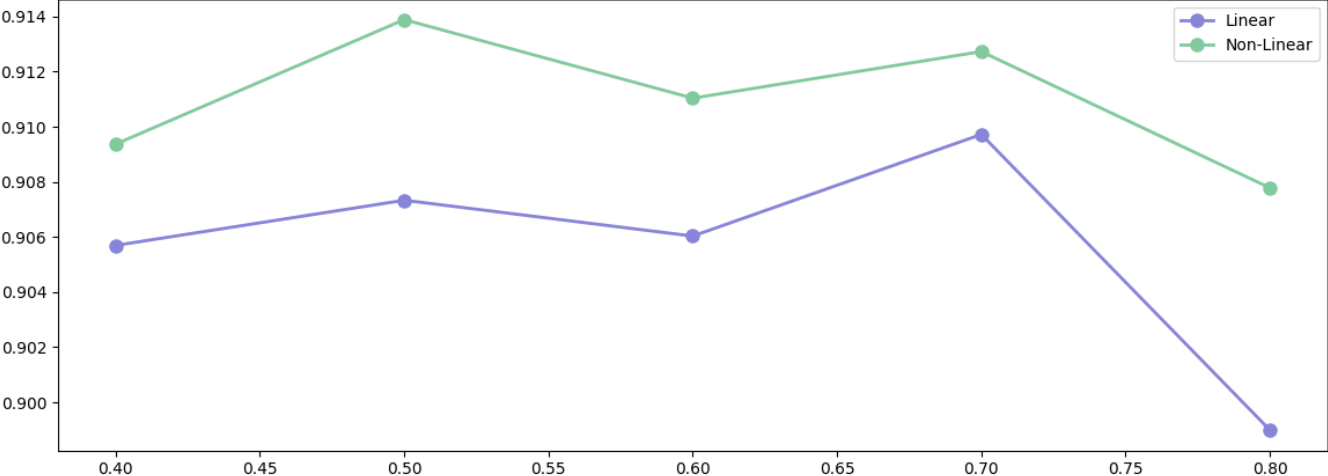
\includegraphics[scale=0.26]{../Images/D_bag.PNG}}
    \caption{Comparison of mean F1-score across the bag size grid when the diabetes dataset is classified by use of 5-fold cross-validation.}
    \label{fig:D_bag_comparison}
\end{figure}
The optimal bag size for the linear and non-linear logistic regression ensemble models is a value of 0.5 and 0.7 respectively,
therefore a larger bag size, such as 0.8 used for the classification of the diabetes dataset decreases the
performance of the linear and non-linear logistic regression ensemble model.

The paired t-test between the two models returned a p-value of 0.0065, which indicates there is a significant difference
between the average F1-scores of the linear and non-linear logistic regression ensembles based on the diabetes dataset.

From figure \ref{fig:D_bag_comparison} it is seen that the non-linear logistic regression ensemble performs best across
all different bag sizes. Therefore the non-linear logistic ensemble model performs best on the diabetes dataset when the
bag size is considered.

\subsubsection{Number of features}

Table \ref{table: D_features_linear_performance_metrics} presents the mean, standard deviation, minimum and maximum of the
F1-scores from the 5-fold cross-validation of the linear logistic regression ensemble, grouped by each number of randomly selected
features value in the grid.
\begin{table}[H]
    \caption{Summary Statistics of F1-Scores for Each Number of Features of the Linear Logistic Regression Ensemble on the Diabetes Dataset}
    \begin{center}
        \begin{tabular}{|c||c|c|c|c|c|}
            \hline
            \textbf{Number of Featurs}&\multicolumn{5}{|c|}{\textbf{Summary Statistics}} \\
            % \textbf{Max depth}
            \cline{2-6}
                       &\textbf{\textit{count}} & \textbf{\textit{mean}} & \textbf{\textit{std}} & \textbf{\textit{min}} & \textbf{\textit{max}}\\
            \hline
            \textbf{\textit{0.4}} & 125 & 88.94 & 0.0218 & 82.96 & 92.87 \\
            \textbf{\textit{0.5}} & 125 & 90.24 & 0.0189 & 85.78 & 93.23 \\
            \textbf{\textit{0.6}} & 125 & 90.96 & 0.0207 & 84.83 & 93.41 \\
            \textbf{\textit{0.7}} & 125 & 91.07 & 0.0212 & 84.83 & 93.39 \\
            \textbf{\textit{0.8}} & 125 & 91.57 & 0.0214 & 86.52 & 94.05 \\
            \hline
        \end{tabular}
    \end{center}
    \label{table: D_features_linear_performance_metrics}
\end{table}
The Kruskal-Wallis test returned a p-value of 0 between the scores of the linear logistic regression ensemble model,
which means there is a significant difference between the scores. Therefore, the number of randomly selected
features has a notable effect on the performance of the linear logistic regression ensemble on the diabetes dataset.

Table \ref{table: D_feature_nonlinear_performance_metrics} presents the mean, standard deviation, minimum and maximum of the
F1-scores from the 5-fold cross-validation of the non-linear logistic regression ensemble, grouped by each number of randomly selected
features value in the grid.
\begin{table}[H]
    \caption{Summary Statistics of F1-Scores for Each Number of Features of the Non-Linear Logistic Regression Ensemble on the Diabetes Dataset}
    \begin{center}
        \begin{tabular}{|c||c|c|c|c|c|}
            \hline
            \textbf{Number of Features}&\multicolumn{5}{|c|}{\textbf{Summary Statistics}} \\
            % \textbf{Max depth}
            \cline{2-6}
                                &\textbf{\textit{count}} & \textbf{\textit{mean}} & \textbf{\textit{std}} & \textbf{\textit{min}} & \textbf{\textit{max}}\\
            \hline
            \textbf{\textit{0.4}} & 125 & 90.02 & 0.0210 & 84.63 & 93.49 \\
            \textbf{\textit{0.5}} & 125 & 91.21 & 0.0205 & 86.12 & 94.00 \\
            \textbf{\textit{0.6}} & 125 & 91.29 & 0.0205 & 86.77 & 93.73 \\
            \textbf{\textit{0.7}} & 125 & 91.34 & 0.0195 & 86.77 & 93.73 \\
            \textbf{\textit{0.8}} & 125 & 91.63 & 0.0192 & 87.24 & 93.90 \\
            \hline
        \end{tabular}
    \end{center}
    \label{table: D_feature_nonlinear_performance_metrics}
\end{table}
The Kruskal-Wallis test returned a p-value of 0 between the scores of the non-linear logistic regression ensemble model,
which means there is a significant difference between the scores. Therefore, the number of randomly selected
features has a notable effect on the performance of the non-linear logistic regression ensemble on the diabetes dataset.

The mean F1-scores obtained from each value of number of randomly selected features in the grid from both the linear and non-linear
logistic regression ensemble models is presented in Figure \ref{fig:D_features_comparison}.
\begin{figure}[H]
    \centerline{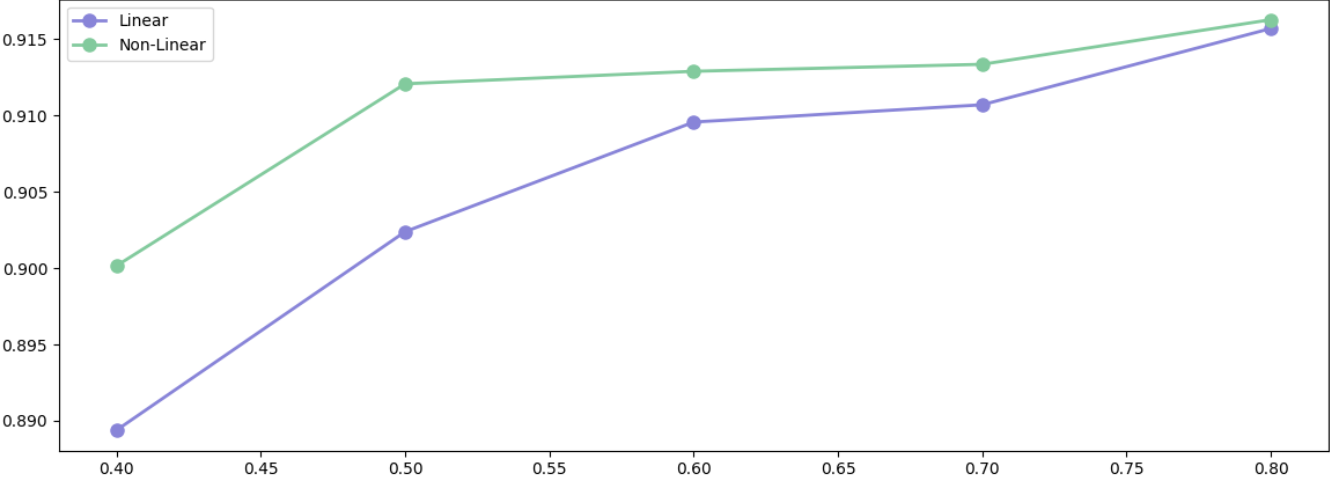
\includegraphics[scale=0.26]{../Images/D_features.PNG}}
    \caption{Comparison of mean F1-score across the number of randomly selected features grid when the diabetes dataset is classified by use of 5-fold cross-validation.}
    \label{fig:D_features_comparison}
\end{figure}
The optimal bag size to use in both the linear and logistic regression ensemble models is 0.8.

The paired t-test between the two models returned a p-value of 0.0462, which indicates there is a significant difference
between the average F1-scores of the linear and non-linear logistic regression ensembles based on the diabetes dataset.

From figure \ref{fig:D_features_comparison} it is seen that the non-linear logistic regression ensemble performs best across
all different number of features. Therefore the non-linear logistic ensemble model performs best on the diabetes dataset when the
number of features is considered.

\subsubsection{Number of ensemble members}

Table \ref{table: D_member_linear_performance_metrics} presents the mean, standard deviation, minimum and maximum of the
F1-scores from the 5-fold cross-validation of the linear logistic regression ensemble, grouped by each number of ensemble members
value in the grid.
\begin{table}[H]
    \caption{Summary Statistics of F1-Scores for Each Number of Ensemble Members of the Linear Logistic Regression Ensemble on the Diabetes Dataset}
    \begin{center}
        \begin{tabular}{|c||c|c|c|c|c|}
            \hline
            \textbf{Number of Featurs}&\multicolumn{5}{|c|}{\textbf{Summary Statistics}} \\
            % \textbf{Max depth}
            \cline{2-6}
                       &\textbf{\textit{count}} & \textbf{\textit{mean}} & \textbf{\textit{std}} & \textbf{\textit{min}} & \textbf{\textit{max}}\\
            \hline
            \textbf{\textit{5}}   & 125 & 90.05 & 0.0242 & 82.96 & 93.68 \\
            \textbf{\textit{10}}  & 125 & 90.60 & 0.0234 & 84.21 & 94.05 \\
            \textbf{\textit{20}}  & 125 & 90.64 & 0.0216 & 84.49 & 94.05 \\
            \textbf{\textit{50}}  & 125 & 90.67 & 0.0222 & 84.41 & 93.89 \\
            \textbf{\textit{100}} & 125 & 90.81 & 0.0215 & 84.41 & 93.86 \\
            \hline
        \end{tabular}
    \end{center}
    \label{table: D_member_linear_performance_metrics}
\end{table}
The Kruskal-Wallis test returned a p-value of 0.0764 between the scores of the linear logistic regression ensemble model,
which means there is no significant difference between the scores. Therefore, the number of ensemble members
has a minimal effect on the performance of the linear logistic regression ensemble on the diabetes dataset.

Table \ref{table: D_member_nonlinear_performance_metrics} presents the mean, standard deviation, minimum and maximum of the
F1-scores from the 5-fold cross-validation of the non-linear logistic regression ensemble, grouped by each number of ensemble members
value in the grid.
\begin{table}[H]
    \caption{Summary Statistics of F1-Scores for Each Number of Ensemble Members of the Non-Linear Logistic Regression Ensemble on the Diabetes Dataset}
    \begin{center}
        \begin{tabular}{|c||c|c|c|c|c|}
            \hline
            \textbf{Number of Features}&\multicolumn{5}{|c|}{\textbf{Summary Statistics}} \\
            % \textbf{Max depth}
            \cline{2-6}
                                &\textbf{\textit{count}} & \textbf{\textit{mean}} & \textbf{\textit{std}} & \textbf{\textit{min}} & \textbf{\textit{max}}\\
            \hline
            \textbf{\textit{5}}   & 125 & 91.17 & 0.0223 & 85.25 & 94. \\
            \textbf{\textit{10}}  & 125 & 91.14 & 0.0212 & 84.63 & 93.88 \\
            \textbf{\textit{20}}  & 125 & 91.07 & 0.0203 & 85.92 & 93.63 \\
            \textbf{\textit{50}}  & 125 & 90.96 & 0.0207 & 85.04 & 93.44 \\
            \textbf{\textit{100}} & 125 & 91.13 & 0.0199 & 85.38 & 93.63 \\
            \hline
        \end{tabular}
    \end{center}
    \label{table: D_member_nonlinear_performance_metrics}
\end{table}
The Kruskal-Wallis test returned a p-value of 0.3451 between the scores of the non-linear logistic regression ensemble model,
which means there is no significant difference between the scores. Therefore, the number of ensemble members
has a minimal effect on the performance of the non-linear logistic regression ensemble on the diabetes dataset.

The mean F1-scores obtained from each value of number of ensemble members in the grid from both the linear and non-linear
logistic regression ensemble models is presented in Figure \ref{fig:D_member_comparison}.
\begin{figure}[H]
    \centerline{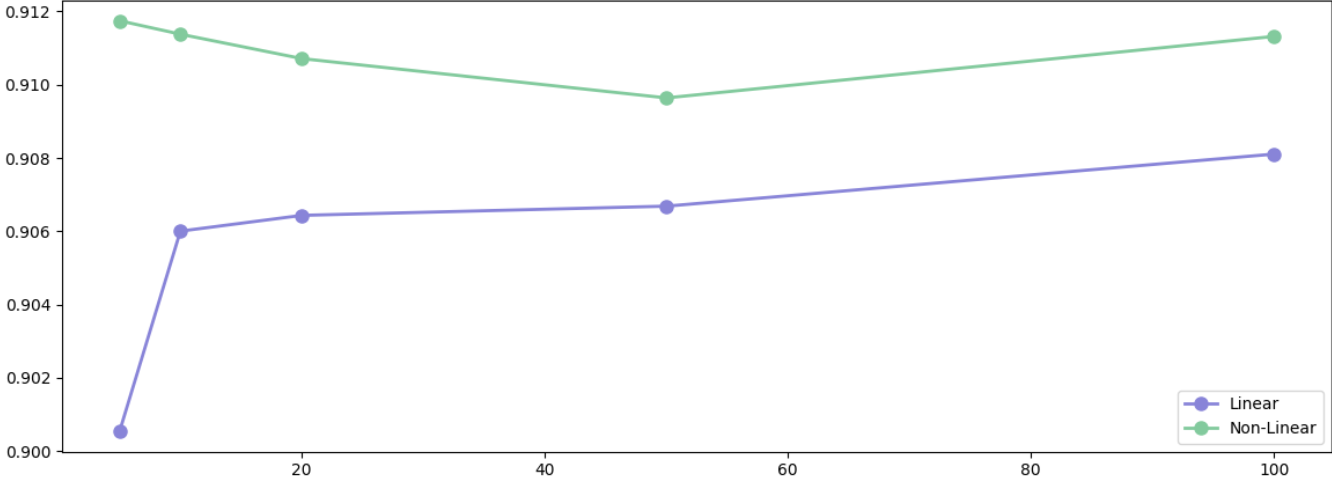
\includegraphics[scale=0.26]{../Images/D_members.PNG}}
    \caption{Comparison of mean F1-score across the number of ensemble members grid when the diabetes dataset is classified by use of 5-fold cross-validation.}
    \label{fig:D_member_comparison}
\end{figure}
The average F1-score of the number of members for the non-linear logistic regression ensemble model starts
to decrease from 10 members and is then more or less the same at 100 members. An optimal value of members for the
non-linear logistic regression ensemble is 5 as the model would train faster and obtain more or less the same results.

The paired t-test between the two models returned a p-value of 0.0233, which indicates there is a significant difference
between the average F1-scores of the linear and non-linear logistic regression ensembles based on the diabetes dataset.

From figure \ref{fig:D_member_comparison} it is seen that the non-linear logistic regression ensemble performs best across
all different number of ensemble members. Therefore the non-linear logistic ensemble model performs best on the diabetes dataset when the
number of ensemble members is considered.

\subsection{Banana Quality Dataset}

By use of Bayesian optimisation, the optimal values of the control parameters in the
linear and non-linear logistic regression ensembles are determined as seen in
Section \ref{section: control_parameters}.

A 5-fold cross validation technique is then applied to the grid search of the linear and non-linear logistic regression ensemble models
to investigate the influence of the size of the bag, the number of randomly selected features and
the number of ensemble members as seen in Section \ref{section: experimental_setup_emp}.

\subsubsection{Bag size}

Table \ref{table: BQ_bagsize_linear_performance_metrics} presents the mean, standard deviation, minimum and maximum of the
accuracy scores from the 5-fold cross-validation of the linear logistic regression ensemble, grouped by each bag size
value in the grid.
\begin{table}[H]
    \caption{Summary Statistics of Accuracy Scores for Each Bag Size of the Linear Logistic Regression Ensemble on the Banana Quality Dataset}
    \begin{center}
        \begin{tabular}{|c||c|c|c|c|c|}
            \hline
            \textbf{Bag Size}&\multicolumn{5}{|c|}{\textbf{Summary Statistics}} \\
            % \textbf{Max depth}
            \cline{2-6}
                       &\textbf{\textit{count}} & \textbf{\textit{mean}} & \textbf{\textit{std}} & \textbf{\textit{min}} & \textbf{\textit{max}}\\
            \hline
            \textbf{\textit{0.4}} & 125 & 85.88 & 0.0196 & 80.44 & 88.81 \\
            \textbf{\textit{0.5}} & 125 & 85.81 & 0.0219 & 79.06 & 88.75 \\
            \textbf{\textit{0.6}} & 125 & 86.58 & 0.0124 & 82.12 & 88.44 \\
            \textbf{\textit{0.7}} & 125 & 84.99 & 0.0449 & 68.81 & 88.69 \\
            \textbf{\textit{0.8}} & 125 & 86.38 & 0.0129 & 82.12 & 88.25 \\
            \hline
        \end{tabular}
    \end{center}
    \label{table: BQ_bagsize_linear_performance_metrics}
\end{table}
The Kruskal-Wallis test returned a p-value of 0.0708 between the scores of the linear logistic regression ensemble model,
which means there is no significant difference between the scores. Therefore, the bag size has a minimal effect on the
performance of the linear logistic regression ensemble on the banana quality dataset.

Table \ref{table: BQ_bagsize_nonlinear_performance_metrics} presents the mean, standard deviation, minimum and maximum of the
accuracy scores from the 5-fold cross-validation of the non-linear logistic regression ensemble, grouped by each bag size
value in the grid.
\begin{table}[H]
    \caption{Summary Statistics of Accuracy Scores for Each Bag Size of the Non-Linear Logistic Regression Ensemble on the Banana Quality Dataset}
    \begin{center}
        \begin{tabular}{|c||c|c|c|c|c|}
            \hline
            \textbf{Bag Size}&\multicolumn{5}{|c|}{\textbf{Summary Statistics}} \\
            % \textbf{Max depth}
            \cline{2-6}
                                &\textbf{\textit{count}} & \textbf{\textit{mean}} & \textbf{\textit{std}} & \textbf{\textit{min}} & \textbf{\textit{max}}\\
            \hline
            \textbf{\textit{0.4}} & 125 & 92.88 & 0.0367 & 81.75 & 97.00 \\
            \textbf{\textit{0.5}} & 125 & 93.09 & 0.0319 & 82.38 & 96.94 \\
            \textbf{\textit{0.6}} & 125 & 94.08 & 0.0269 & 87.00 & 97.06 \\
            \textbf{\textit{0.7}} & 125 & 92.00 & 0.0613 & 69.50 & 97.12 \\
            \textbf{\textit{0.8}} & 125 & 92.46 & 0.0435 & 71.00 & 96.88 \\
            \hline
        \end{tabular}
    \end{center}
    \label{table: BQ_bagsize_nonlinear_performance_metrics}
\end{table}
The Kruskal-Wallis test returned a p-value of 0.0056 between the scores of the non-linear logistic regression ensemble model,
which means there is a significant difference between the scores. Therefore, the bag size has a notable effect on the
performance of the non-linear logistic regression ensemble on the banana quality dataset.

The mean accuracy scores obtained from each value of bag size in the grid from both the linear and non-linear
logistic regression ensemble models is presented in Figure \ref{fig:BQ_bag_comparison}.
\begin{figure}[H]
    \centerline{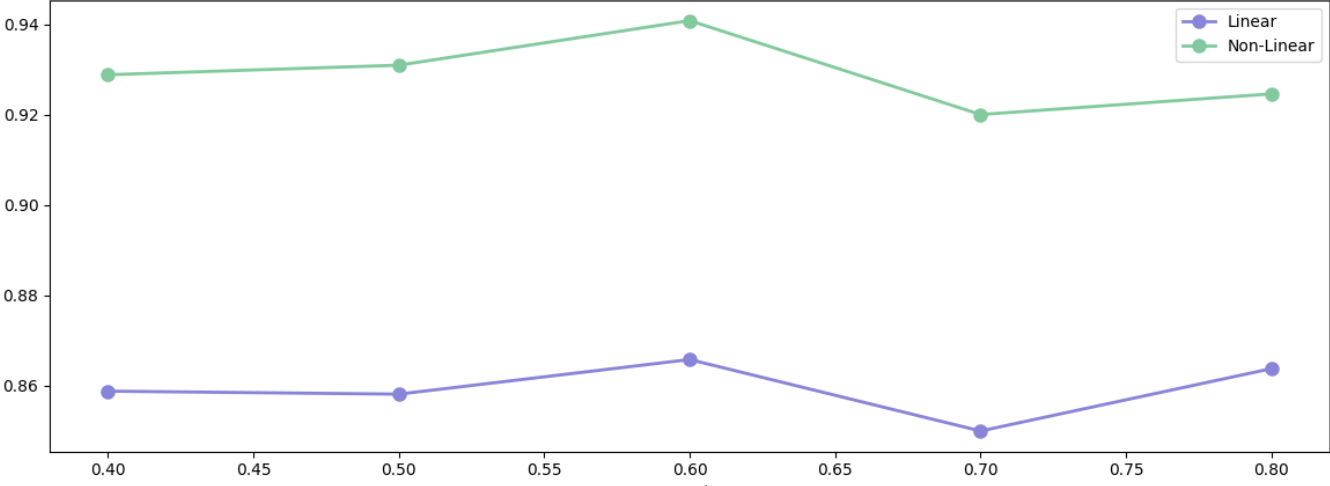
\includegraphics[scale=0.26]{../Images/BQ_bag.PNG}}
    \caption{Comparison of mean accuracy score across the bag size grid when the banana quality dataset is classified by use of 5-fold cross-validation.}
    \label{fig:BQ_bag_comparison}
\end{figure}
The optimal bag size for the linear and non-linear logistic regression ensemble models is a value of 0.6.
Both models predictions also become inconsistent for a bag size larger than 0.6, as the minimum average
accuracy score for a bag size of 0.7 is 68.81\% and 69.5\% for the linear and non-linear logistic regression
ensemble, respectively.

The paired t-test between the two models returned a p-value of 0, which indicates there is a significant difference
between the average accuracy scores of the linear and non-linear logistic regression ensembles based on the banana
quality dataset.

From figure \ref{fig:BQ_bag_comparison} it is seen that the non-linear logistic regression ensemble performs best across
all different bag sizes. Therefore the non-linear logistic ensemble model performs best on the banana quality dataset when the
bag size is considered.

\subsubsection{Number of features}

Table \ref{table: BQ_features_linear_performance_metrics} presents the mean, standard deviation, minimum and maximum of the
accuracy scores from the 5-fold cross-validation of the linear logistic regression ensemble, grouped by each number of randomly selected
features value in the grid.
\begin{table}[H]
    \caption{Summary Statistics of Accuracy Scores for Each Number of Features of the Linear Logistic Regression Ensemble on the Banana Quality Dataset}
    \begin{center}
        \begin{tabular}{|c||c|c|c|c|c|}
            \hline
            \textbf{Number of Featurs}&\multicolumn{5}{|c|}{\textbf{Summary Statistics}} \\
            % \textbf{Max depth}
            \cline{2-6}
                       &\textbf{\textit{count}} & \textbf{\textit{mean}} & \textbf{\textit{std}} & \textbf{\textit{min}} & \textbf{\textit{max}}\\
            \hline
            \textbf{\textit{0.4}} & 125 & 84.69 & 0.0367 & 68.81 & 88.19 \\
            \textbf{\textit{0.5}} & 125 & 85.45 & 0.0282 & 73.44 & 88.75 \\
            \textbf{\textit{0.6}} & 125 & 86.11 & 0.0197 & 78.56 & 88.81 \\
            \textbf{\textit{0.7}} & 125 & 86.11 & 0.0197 & 78.56 & 88.81 \\
            \textbf{\textit{0.8}} & 125 & 87.27 & 0.0078 & 84.12 & 88.75 \\
            \hline
        \end{tabular}
    \end{center}
    \label{table: BQ_features_linear_performance_metrics}
\end{table}
The Kruskal-Wallis test returned a p-value of 0 between the scores of the linear logistic regression ensemble model,
which means there is a significant difference between the scores. Therefore, the number of randomly selected
features has a notable effect on the performance of the linear logistic regression ensemble on the banana quality dataset.

Table \ref{table: BQ_feature_nonlinear_performance_metrics} presents the mean, standard deviation, minimum and maximum of the
accuracy scores from the 5-fold cross-validation of the non-linear logistic regression ensemble, grouped by each number of randomly selected
features value in the grid.
\begin{table}[H]
    \caption{Summary Statistics of Accuracy Scores for Each Number of Features of the Non-Linear Logistic Regression Ensemble on the Banana Quality Dataset}
    \begin{center}
        \begin{tabular}{|c||c|c|c|c|c|}
            \hline
            \textbf{Number of Features}&\multicolumn{5}{|c|}{\textbf{Summary Statistics}} \\
            % \textbf{Max depth}
            \cline{2-6}
                                &\textbf{\textit{count}} & \textbf{\textit{mean}} & \textbf{\textit{std}} & \textbf{\textit{min}} & \textbf{\textit{max}}\\
            \hline
            \textbf{\textit{0.4}} & 125 & 87.22 & 0.0493 & 69.50 & 93.69 \\
            \textbf{\textit{0.5}} & 125 & 91.89 & 0.0328 & 72.88 & 95.31 \\
            \textbf{\textit{0.6}} & 125 & 94.58 & 0.0142 & 89.62 & 96.75 \\
            \textbf{\textit{0.7}} & 125 & 94.58 & 0.0142 & 89.62 & 96.75 \\
            \textbf{\textit{0.8}} & 125 & 96.24 & 0.0049 & 94.56 & 97.12 \\
            \hline
        \end{tabular}
    \end{center}
    \label{table: BQ_feature_nonlinear_performance_metrics}
\end{table}
The Kruskal-Wallis test returned a p-value of 0 between the scores of the non-linear logistic regression ensemble model,
which means there is a significant difference between the scores. Therefore, the number of randomly selected
features has a notable effect on the performance of the non-linear logistic regression ensemble on the banana quality dataset.

The mean accuracy scores obtained from each value of number of randomly selected features in the grid from both the linear and non-linear
logistic regression ensemble models is presented in Figure \ref{fig:BQ_features_comparison}.
\begin{figure}[H]
    \centerline{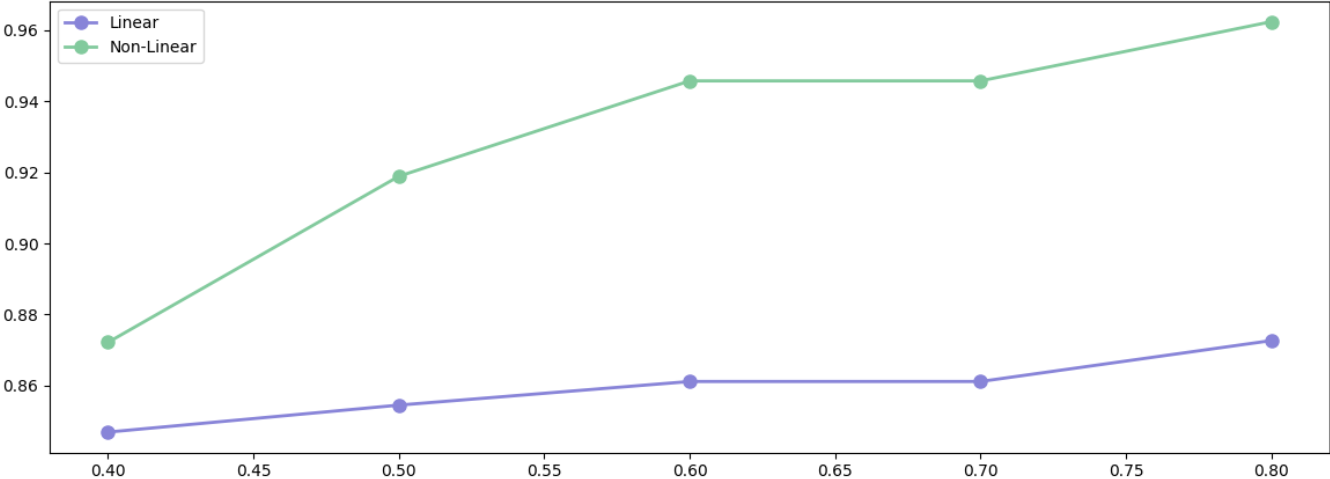
\includegraphics[scale=0.26]{../Images/BQ_features.PNG}}
    \caption{Comparison of mean accuracy score across the number of randomly selected features grid when the banana quality dataset is classified by use of 5-fold cross-validation.}
    \label{fig:BQ_features_comparison}
\end{figure}
The optimal value for the number of features in the linear and non-linear logistic regression ensemble is 0.8, which indicates
that both models performs better when constructed on more features.

The paired t-test between the two models returned a p-value of 0.0043, which indicates there is a significant difference
between the average accuracy scores of the linear and non-linear logistic regression ensembles based on the banana quality dataset.

From figure \ref{fig:BQ_features_comparison} it is seen that the non-linear logistic regression ensemble performs best across
all different number of features. Therefore the non-linear logistic ensemble model performs best on the banana quality dataset when the
number of features is considered.

\subsubsection{Number of ensemble members}

Table \ref{table: BQ_member_linear_performance_metrics} presents the mean, standard deviation, minimum and maximum of the
accuracy scores from the 5-fold cross-validation of the linear logistic regression ensemble, grouped by each number of ensemble members
value in the grid.
\begin{table}[H]
    \caption{Summary Statistics of Accuracy Scores for Each Number of Ensemble Members of the Linear Logistic Regression Ensemble on the Banana Quality Dataset}
    \begin{center}
        \begin{tabular}{|c||c|c|c|c|c|}
            \hline
            \textbf{Number of Featurs}&\multicolumn{5}{|c|}{\textbf{Summary Statistics}} \\
            % \textbf{Max depth}
            \cline{2-6}
                       &\textbf{\textit{count}} & \textbf{\textit{mean}} & \textbf{\textit{std}} & \textbf{\textit{min}} & \textbf{\textit{max}}\\
            \hline
            \textbf{\textit{5}}   & 125 & 82.90 & 0.0393 & 68.81 & 88.31 \\
            \textbf{\textit{10}}  & 125 & 85.74 & 0.0169 & 79.94 & 88.75 \\
            \textbf{\textit{20}}  & 125 & 86.66 & 0.0111 & 82.12 & 88.69 \\
            \textbf{\textit{50}}  & 125 & 87.08 & 0.0074 & 85.38 & 88.81 \\
            \textbf{\textit{100}} & 125 & 87.26 & 0.0065 & 85.62 & 88.75 \\
            \hline
        \end{tabular}
    \end{center}
    \label{table: BQ_member_linear_performance_metrics}
\end{table}
The Kruskal-Wallis test returned a p-value of 0 between the scores of the linear logistic regression ensemble model,
which means there is a significant difference between the scores. Therefore, the number of ensemble members
has a notable effect on the performance of the linear logistic regression ensemble on the banana quality dataset.

Table \ref{table: BQ_member_nonlinear_performance_metrics} presents the mean, standard deviation, minimum and maximum of the
accuracy scores from the 5-fold cross-validation of the non-linear logistic regression ensemble, grouped by each number of ensemble members
value in the grid.
\begin{table}[H]
    \caption{Summary Statistics of Accuracy Scores for Each Number of Ensemble Members of the Non-Linear Logistic Regression Ensemble on the Banana Quality Dataset}
    \begin{center}
        \begin{tabular}{|c||c|c|c|c|c|}
            \hline
            \textbf{Number of Features}&\multicolumn{5}{|c|}{\textbf{Summary Statistics}} \\
            % \textbf{Max depth}
            \cline{2-6}
                                &\textbf{\textit{count}} & \textbf{\textit{mean}} & \textbf{\textit{std}} & \textbf{\textit{min}} & \textbf{\textit{max}}\\
            \hline
            \textbf{\textit{5}}   & 125 & 90.15 & 0.0627 & 69.50 & 96.75 \\
            \textbf{\textit{10}}  & 125 & 92.18 & 0.0423 & 71.00 & 96.69 \\
            \textbf{\textit{20}}  & 125 & 93.36 & 0.0305 & 82.88 & 96.88 \\
            \textbf{\textit{50}}  & 125 & 94.16 & 0.0235 & 87.75 & 97.00 \\
            \textbf{\textit{100}} & 125 & 94.66 & 0.0219 & 88.31 & 97.12 \\
            \hline
        \end{tabular}
    \end{center}
    \label{table: BQ_member_nonlinear_performance_metrics}
\end{table}
The Kruskal-Wallis test returned a p-value of 0 between the scores of the non-linear logistic regression ensemble model,
which means there is a significant difference between the scores. Therefore, the number of ensemble members
has a notable effect on the performance of the non-linear logistic regression ensemble on the banana quality dataset.

The mean accuracy scores obtained from each value of number of ensemble members in the grid from both the linear and non-linear
logistic regression ensemble models is presented in Figure \ref{fig:BQ_member_comparison}.
\begin{figure}[H]
    \centerline{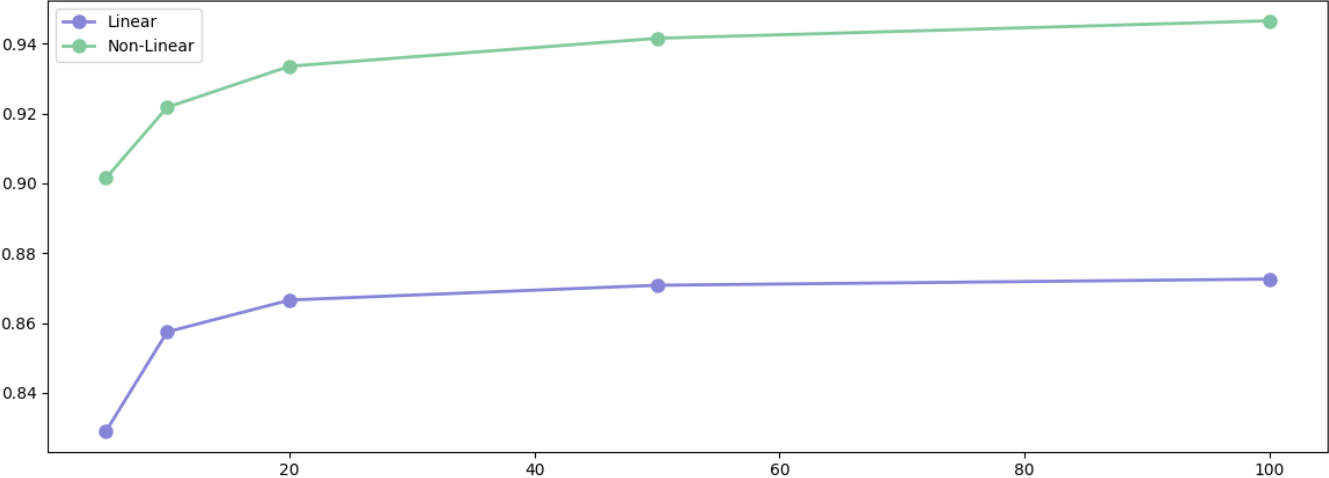
\includegraphics[scale=0.26]{../Images/BQ_members.PNG}}
    \caption{Comparison of mean accuracy score across the number of ensemble members grid when the banana quality dataset is classified by use of 5-fold cross-validation.}
    \label{fig:BQ_member_comparison}
\end{figure}
From 20 members in both the linear and non-linear logistic regression ensemble models, the average accuracy score
increases by a very small amount. To allow the model to train faster, an optimal value of 20 members is chosen for
both ensemble models.

The paired t-test between the two models returned a p-value of 0, which indicates there is a significant difference
between the average accuracy scores of the linear and non-linear logistic regression ensembles based on the banana quality dataset.

From figure \ref{fig:BQ_member_comparison} it is seen that the non-linear logistic regression ensemble performs best across
all different number of ensemble members. Therefore the non-linear logistic ensemble model performs best on the banana quality dataset when the
number of ensemble members is considered.

\subsection{Spiral Dataset}

By use of Bayesian optimisation, the optimal values of the control parameters in the
linear and non-linear logistic regression ensembles are determined as seen in
Section \ref{section: control_parameters}.

A 5-fold cross validation technique is then applied to the grid search of the linear and non-linear logistic regression ensemble models
to investigate the influence of the size of the bag and the number of ensemble members as seen in Section \ref{section: experimental_setup_emp}.

\subsubsection{Bag size}

Table \ref{table: S_bagsize_linear_performance_metrics} presents the mean, standard deviation, minimum and maximum of the
accuracy scores from the 5-fold cross-validation of the linear logistic regression ensemble, grouped by each bag size
value in the grid.
\begin{table}[H]
    \caption{Summary Statistics of Accuracy Scores for Each Bag Size of the Linear Logistic Regression Ensemble on the Spiral Dataset}
    \begin{center}
        \begin{tabular}{|c||c|c|c|c|c|}
            \hline
            \textbf{Bag Size}&\multicolumn{5}{|c|}{\textbf{Summary Statistics}} \\
            % \textbf{Max depth}
            \cline{2-6}
                       &\textbf{\textit{count}} & \textbf{\textit{mean}} & \textbf{\textit{std}} & \textbf{\textit{min}} & \textbf{\textit{max}}\\
            \hline
            \textbf{\textit{0.4}} & 25 & 59.31 & 0.0259 & 54.4 & 62 \\
            \textbf{\textit{0.5}} & 25 & 59.65 & 0.0278 & 54.4 & 63.2 \\
            \textbf{\textit{0.6}} & 25 & 59.25 & 0.0274 & 54 & 62.8 \\
            \textbf{\textit{0.7}} & 25 & 59.46 & 0.0319 & 54 & 63.6 \\
            \textbf{\textit{0.8}} & 25 & 59.58 & 0.0294 & 54 & 63.6 \\
            \hline
        \end{tabular}
    \end{center}
    \label{table: S_bagsize_linear_performance_metrics}
\end{table}
The Kruskal-Wallis test returned a p-value of 0.8946 between the scores of the linear logistic regression ensemble model,
which means there is no significant difference between the scores. Therefore, the bag size has a minimal effect on the
performance of the linear logistic regression ensemble on the spiral dataset.

Table \ref{table: S_bagsize_nonlinear_performance_metrics} presents the mean, standard deviation, minimum and maximum of the
accuracy scores from the 5-fold cross-validation of the non-linear logistic regression ensemble, grouped by each bag size
value in the grid.
\begin{table}[H]
    \caption{Summary Statistics of Accuracy Scores for Each Bag Size of the Non-Linear Logistic Regression Ensemble on the Spiral Dataset}
    \begin{center}
        \begin{tabular}{|c||c|c|c|c|c|}
            \hline
            \textbf{Bag Size}&\multicolumn{5}{|c|}{\textbf{Summary Statistics}} \\
            % \textbf{Max depth}
            \cline{2-6}
                                &\textbf{\textit{count}} & \textbf{\textit{mean}} & \textbf{\textit{std}} & \textbf{\textit{min}} & \textbf{\textit{max}}\\
            \hline
            \textbf{\textit{0.4}} & 25 & 60.66 & 0.0347 & 54.4 & 64.4 \\
            \textbf{\textit{0.5}} & 25 & 60.69 & 0.0358 & 53.2 & 64.8 \\
            \textbf{\textit{0.6}} & 25 & 61.20 & 0.0368 & 54 & 65.6 \\
            \textbf{\textit{0.7}} & 25 & 61.26 & 0.0368 & 54 & 66.4 \\
            \textbf{\textit{0.8}} & 25 & 62.02 & 0.0383 & 54 & 66.8 \\
            \hline
        \end{tabular}
    \end{center}
    \label{table: S_bagsize_nonlinear_performance_metrics}
\end{table}
The Kruskal-Wallis test returned a p-value of 0.3408 between the scores of the non-linear logistic regression ensemble model,
which means there is no significant difference between the scores. Therefore, the bag size has a minimal effect on the
performance of the non-linear logistic regression ensemble on the spiral dataset.

The mean accuracy scores obtained from each value of bag size in the grid from both the linear and non-linear
logistic regression ensemble models is presented in Figure \ref{fig:S_bag_comparison}.
\begin{figure}[H]
    \centerline{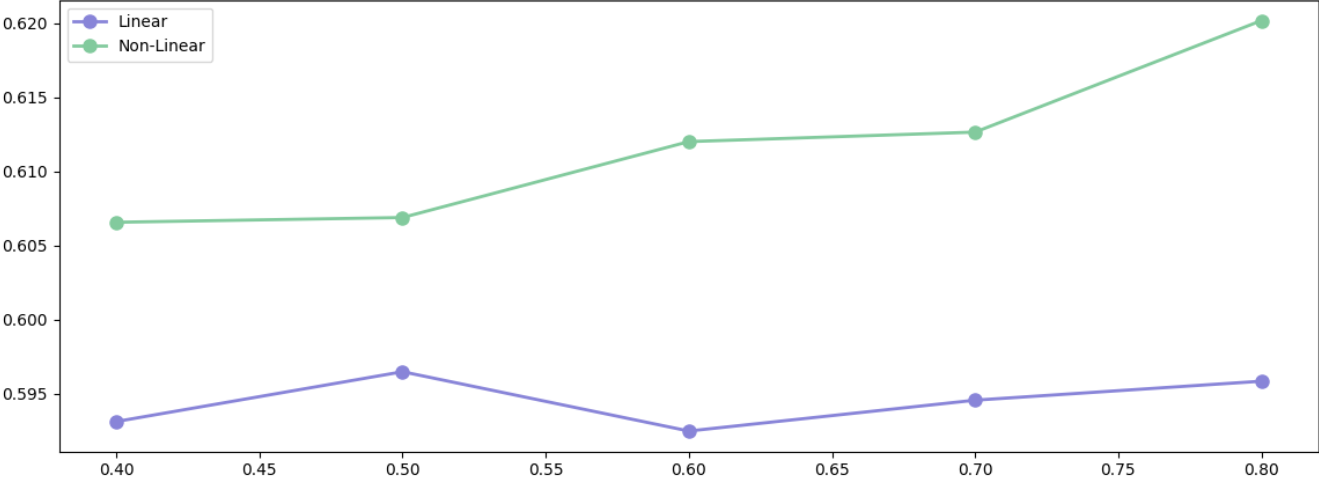
\includegraphics[scale=0.26]{../Images/S_bag.PNG}}
    \caption{Comparison of mean accuracy score across the bag size grid when the spiral dataset is classified by use of 5-fold cross-validation.}
    \label{fig:S_bag_comparison}
\end{figure}
The optimal bag size for the linear and non-linear logistic regression ensemble models is a value of 0.8.

The paired t-test between the two models returned a p-value of 0.0021, which indicates there is a significant difference
between the average accuracy scores of the linear and non-linear logistic regression ensembles based on the spiral dataset.

From figure \ref{fig:S_bag_comparison} it is seen that the non-linear logistic regression ensemble performs best across
all different bag sizes. Therefore the non-linear logistic ensemble model performs best on the spiral dataset when the
bag size is considered.

\subsubsection{Number of ensemble members}

Table \ref{table: S_member_linear_performance_metrics} presents the mean, standard deviation, minimum and maximum of the
accuracy scores from the 5-fold cross-validation of the linear logistic regression ensemble, grouped by each number of ensemble members
value in the grid.
\begin{table}[H]
    \caption{Summary Statistics of Accuracy Scores for Each Number of Ensemble Members of the Linear Logistic Regression Ensemble on the Spiral Dataset}
    \begin{center}
        \begin{tabular}{|c||c|c|c|c|c|}
            \hline
            \textbf{Number of Featurs}&\multicolumn{5}{|c|}{\textbf{Summary Statistics}} \\
            % \textbf{Max depth}
            \cline{2-6}
                       &\textbf{\textit{count}} & \textbf{\textit{mean}} & \textbf{\textit{std}} & \textbf{\textit{min}} & \textbf{\textit{max}}\\
            \hline
            \textbf{\textit{5}}   & 25 & 59.46 & 0.0296 & 54 & 63.6 \\
            \textbf{\textit{10}}  & 25 & 59.34 & 0.0274 & 54 & 63.2 \\
            \textbf{\textit{20}}  & 25 & 59.68 & 0.0298 & 54 & 63.6 \\
            \textbf{\textit{50}}  & 25 & 59.49 & 0.0281 & 54 & 62 \\
            \textbf{\textit{100}} & 25 & 59.28 & 0.0278 & 54 & 62 \\
            \hline
        \end{tabular}
    \end{center}
    \label{table: S_member_linear_performance_metrics}
\end{table}
The Kruskal-Wallis test returned a p-value of 0.9572 between the scores of the linear logistic regression ensemble model,
which means there is no significant difference between the scores. Therefore, the number of ensemble members
has a minimal effect on the performance of the linear logistic regression ensemble on the spiral dataset.

Table \ref{table: S_member_nonlinear_performance_metrics} presents the mean, standard deviation, minimum and maximum of the
accuracy scores from the 5-fold cross-validation of the non-linear logistic regression ensemble, grouped by each number of ensemble members
value in the grid.
\begin{table}[H]
    \caption{Summary Statistics of Accuracy Scores for Each Number of Ensemble Members of the Non-Linear Logistic Regression Ensemble on the Spiral Dataset}
    \begin{center}
        \begin{tabular}{|c||c|c|c|c|c|}
            \hline
            \textbf{Number of Features}&\multicolumn{5}{|c|}{\textbf{Summary Statistics}} \\
            % \textbf{Max depth}
            \cline{2-6}
                                &\textbf{\textit{count}} & \textbf{\textit{mean}} & \textbf{\textit{std}} & \textbf{\textit{min}} & \textbf{\textit{max}}\\
            \hline
            \textbf{\textit{5}}   & 25 & 60.69 & 0.0320 & 54 & 66.4 \\
            \textbf{\textit{10}}  & 25 & 61.14 & 0.0334 & 54.8 & 64.8 \\
            \textbf{\textit{20}}  & 25 & 61.09 & 0.0363 & 54 & 64.4 \\
            \textbf{\textit{50}}  & 25 & 61.65 & 0.0411 & 53.2 & 66.8 \\
            \textbf{\textit{100}} & 25 & 61.26 & 0.0399 & 54.4 & 65.6 \\
            \hline
        \end{tabular}
    \end{center}
    \label{table: S_member_nonlinear_performance_metrics}
\end{table}
The Kruskal-Wallis test returned a p-value of 0.4160 between the scores of the non-linear logistic regression ensemble model,
which means there is no significant difference between the scores. Therefore, the number of ensemble members
has a minimal effect on the performance of the non-linear logistic regression ensemble on the spiral dataset.

The mean accuracy scores obtained from each value of number of ensemble members in the grid from both the linear and non-linear
logistic regression ensemble models is presented in Figure \ref{fig:S_member_comparison}.
\begin{figure}[H]
    \centerline{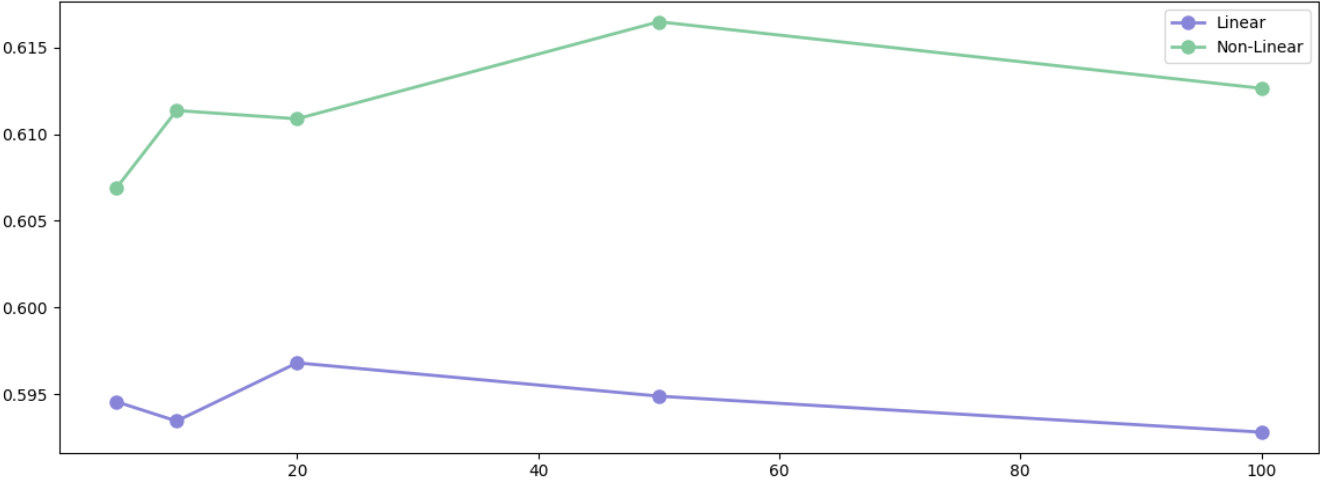
\includegraphics[scale=0.26]{../Images/S_members.PNG}}
    \caption{Comparison of mean accuracy score across the number of ensemble members grid when the spiral dataset is classified by use of 5-fold cross-validation.}
    \label{fig:S_member_comparison}
\end{figure}
The optimal number of members for both of the linear and non-linear logistic regression ensembles is 20 and 50 respectively.

The paired t-test between the two models returned a p-value of 0.0006, which indicates there is a significant difference
between the average accuracy scores of the linear and non-linear logistic regression ensembles based on the spiral dataset.

From figure \ref{fig:S_member_comparison} it is seen that the non-linear logistic regression ensemble performs best across
all different number of ensemble members. Therefore the non-linear logistic ensemble model performs best on the spiral dataset when the
number of ensemble members is considered.

\section{Conclusion} \label{section: Conclusion}

This paper investigated the influence of the size of the bags, the number of randomly selected features and
the number of members in linear and non-linear logistic regression ensemble models across five binary classification
datasets that varies in complexity. The results show that each factor plays a critical role in model performance,
however, the degree of impact varies based on the complexity of the dataset and the type of model used.

The results indicated the number of statistically significant tests associated with each model configuration.
Specifically, the linear model configuration with a bag size of 2, 3 features, and 1 model showed a lower
count of significant tests, while the non-linear configuration with a bag size of 4, 4 features, and 3
models resulted in a higher count of significant tests across the datasets. To create an optimal ensemble on each
dataset, the size of the bags, the number of randomly selected features, and the number of members should all
be considered together. All of these elements significantly influence how well the ensemble performs.

The non-linear logistic regression ensemble performed the best on all but one of the datasets across all
bag sizes, numbers of randomly selected features, and ensemble members. This consistency in performance
suggests that non-linear ensembles are more adept at capturing complex patterns and interactions within
the data.

\begin{thebibliography}{00}
    \bibitem{Ionosphere_ref} K. Baker, V. Sigillito, S. Wing and L. Hutton "Ionosphere," In: UCI Machine Learning Repository (1989) Available: https://doi.org/10.24432/C5W01B.
    \bibitem{Performance_ref} J. Braet, M. Cristina, Hinojosa-Lee, and J. Springael. "Evaluating performance metrics in emotion lexicon distillation: a focus on F1 scores." (2024).
    \bibitem{Bagging_ref} L. Breiman "Bagging predictors." In: Machine learning (1996).
    \bibitem{gradient_descent_ref} A. Cauchy "Méthode générale pour la résolution des systemes d’équations simultanées." In: Comp. Rend. Sci. Paris (1847).
    \bibitem{logistic_regression_ref} D. R. Cox "The regression analysis of binary sequences." In: Journal of the Royal Statistical Society Series B: Statistical Methodology (1958).
    \bibitem{basis_fun_ref} A. D'arcy, B. Mac Namee, and J. D. Kelleher "Fundamentals of machine learning for predictive data analytics: algorithms, worked examples, and case studies." In: MIT press (2020).
    \bibitem{F1-score_ref} B. J. Erickson, and K. Felipe "Magician’s corner: 9. Performance metrics for machine learning models." In: Radiology: Artificial Intelligence 3(2021).
    \bibitem{Ensemble_ref} M. A. Ganaie, M., Hu, A. K. Malik, M. Tanveer and P. N. Suganthan "Ensemble deep learning: A review." In: Engineering Applications of Artificial Intelligence (2022).
    \bibitem{Diabetes_ref} Y. Chen, X. P. Zhang, J. Yuan, et al "Association of body mass index and age with incident diabetes in Chinese adults: a population-based cohort study" (2018) Available: https://doi.org/10.5061/dryad.ft8750v.
    \bibitem{Breast_cancer_ref} O. Mangasarian, W. Wolberg, N. Street, and W. Street "Breast Cancer Wisconsin (Diagnostic)" In: UCI Machine Learning Repository (1993) Available: https://doi.org/10.24432/C5DW2B.
    \bibitem{Voting_ref} Z. H. Zhou "Ensemble methods: foundations and algorithms." In: CRC press (2012).
    \bibitem{Banana_ref} "Banana Quality" In: Kaggle (2024) Available: https://www.kaggle.com/datasets/l3llff/banana.
\end{thebibliography}

\printglossary[type=\acronymtype]


\end{document}